\documentclass[11pt]{article}
	\usepackage[T1]{fontenc}
    % Nicer default font (+ math font) than Computer Modern for most use cases
    % \usepackage{mathpazo}

    % Basic figure setup, for now with no caption control since it's done
    % automatically by Pandoc (which extracts ![](path) syntax from Markdown).
    \usepackage{graphics}
    % We will generate all images so they have a width \maxwidth. This means
    % that they will get their normal width if they fit onto the page, but
    % are scaled down if they would overflow the margins.
    \makeatletter
    \def\maxwidth{\ifdim\Gin@nat@width>\linewidth\linewidth
    \else\Gin@nat@width\fi}
    \makeatother
    \let\Oldincludegraphics\includegraphics
    % Set max figure width to be 80% of text width, for now hardcoded.
    \renewcommand{\includegraphics}[1]{\Oldincludegraphics[width=.8\maxwidth]{#1}}
    % Ensure that by default, figures have no caption (until we provide a
    % proper Figure object with a Caption API and a way to capture that
    % in the conversion process - todo).
    \usepackage[center,bf]{caption}
    % \DeclareCaptionLabelFormat{nolabel}{}
    % \captionsetup{labelformat=nolabel}

    \usepackage{adjustbox} % Used to constrain images to a maximum size 
    \usepackage{xcolor} % Allow colors to be defined
    \usepackage{enumerate} % Needed for markdown enumerations to work
    \usepackage{geometry} % Used to adjust the document margins
    \usepackage{amsmath} % Equations
    \usepackage{amssymb} % Equations
    \usepackage{textcomp} % defines textquotesingle
    % Hack from http://tex.stackexchange.com/a/47451/13684:
    \AtBeginDocument{%
        \def\PYZsq{\textquotesingle}% Upright quotes in Pygmentized code
    }
    \usepackage{upquote} % Upright quotes for verbatim code
    \usepackage{eurosym} % defines \euro
    \usepackage[mathletters]{ucs} % Extended unicode (utf-8) support
    \usepackage[utf8x]{inputenc} % Allow utf-8 characters in the tex document
    \usepackage{fancyvrb} % verbatim replacement that allows latex
    \usepackage{grffile} % extends the file name processing of package graphics 
                         % to support a larger range 
    % The hyperref package gives us a pdf with properly built
    % internal navigation ('pdf bookmarks' for the table of contents,
    % internal cross-reference links, web links for URLs, etc.)
    \usepackage{hyperref}
    \usepackage{longtable} % longtable support required by pandoc >1.10
    \usepackage{booktabs}  % table support for pandoc > 1.12.2
    \usepackage[inline]{enumitem} % IRkernel/repr support (it uses the enumerate* environment)
    \usepackage[normalem]{ulem} % ulem is needed to support strikethroughs (\sout)
                                % normalem makes italics be italics, not underlines
   	\usepackage[]{authblk}
   	\usepackage{cite}
    \usepackage{graphicx}
    \usepackage{hyperref}
    \usepackage{amsmath}
    \usepackage{amsthm}
    \usepackage{amssymb}
    \usepackage{bm}
    \usepackage{bbm}
    \usepackage{algorithmicx}
    \usepackage{algorithm}
    \usepackage{algpseudocode}
    \usepackage{array}
    \usepackage{booktabs}
    \usepackage{multirow}
    \usepackage{makecell}
    \usepackage{color}
    \usepackage{tabularx,ragged2e,booktabs,caption}

   	\makeatletter
    \def\@maketitle{%
    \newpage
      \null
      \vskip 2em%
      \begin{center}%
      \let \footnote \thanks
        {\Large\bfseries \@title \par}%
        \vskip 1.5em%
        {\normalsize
          \lineskip .5em%
          \begin{tabular}[t]{c}%
            \@author
          \end{tabular}\par}%
        \vskip 1em%
        {\normalsize \@date}%
      \end{center}%
      \par
      \vskip 1.5em}
    \makeatother


\newtheorem{theorem}{Theorem}






\title{EE 232E Project 2\\Social Network Mining}
\author{Hengjie~Yang, Sheng~Chang, Wandi~Cui, and Tianyi~Liu
}


\date{\today}


\begin{document}
\maketitle

% \section{A brief tutorial on how to use this template}
% \Large\textcolor{red}{\bf{Please remove the tutorial section in the final manuscript\\ by commenting, i.e. $\%(something)$}}


% \subsection{Figures}
% Figure insertion is shown in Fig \ref{example_fig}.
% \begin{figure}[h]
% \centering
% \scalebox{0.7}{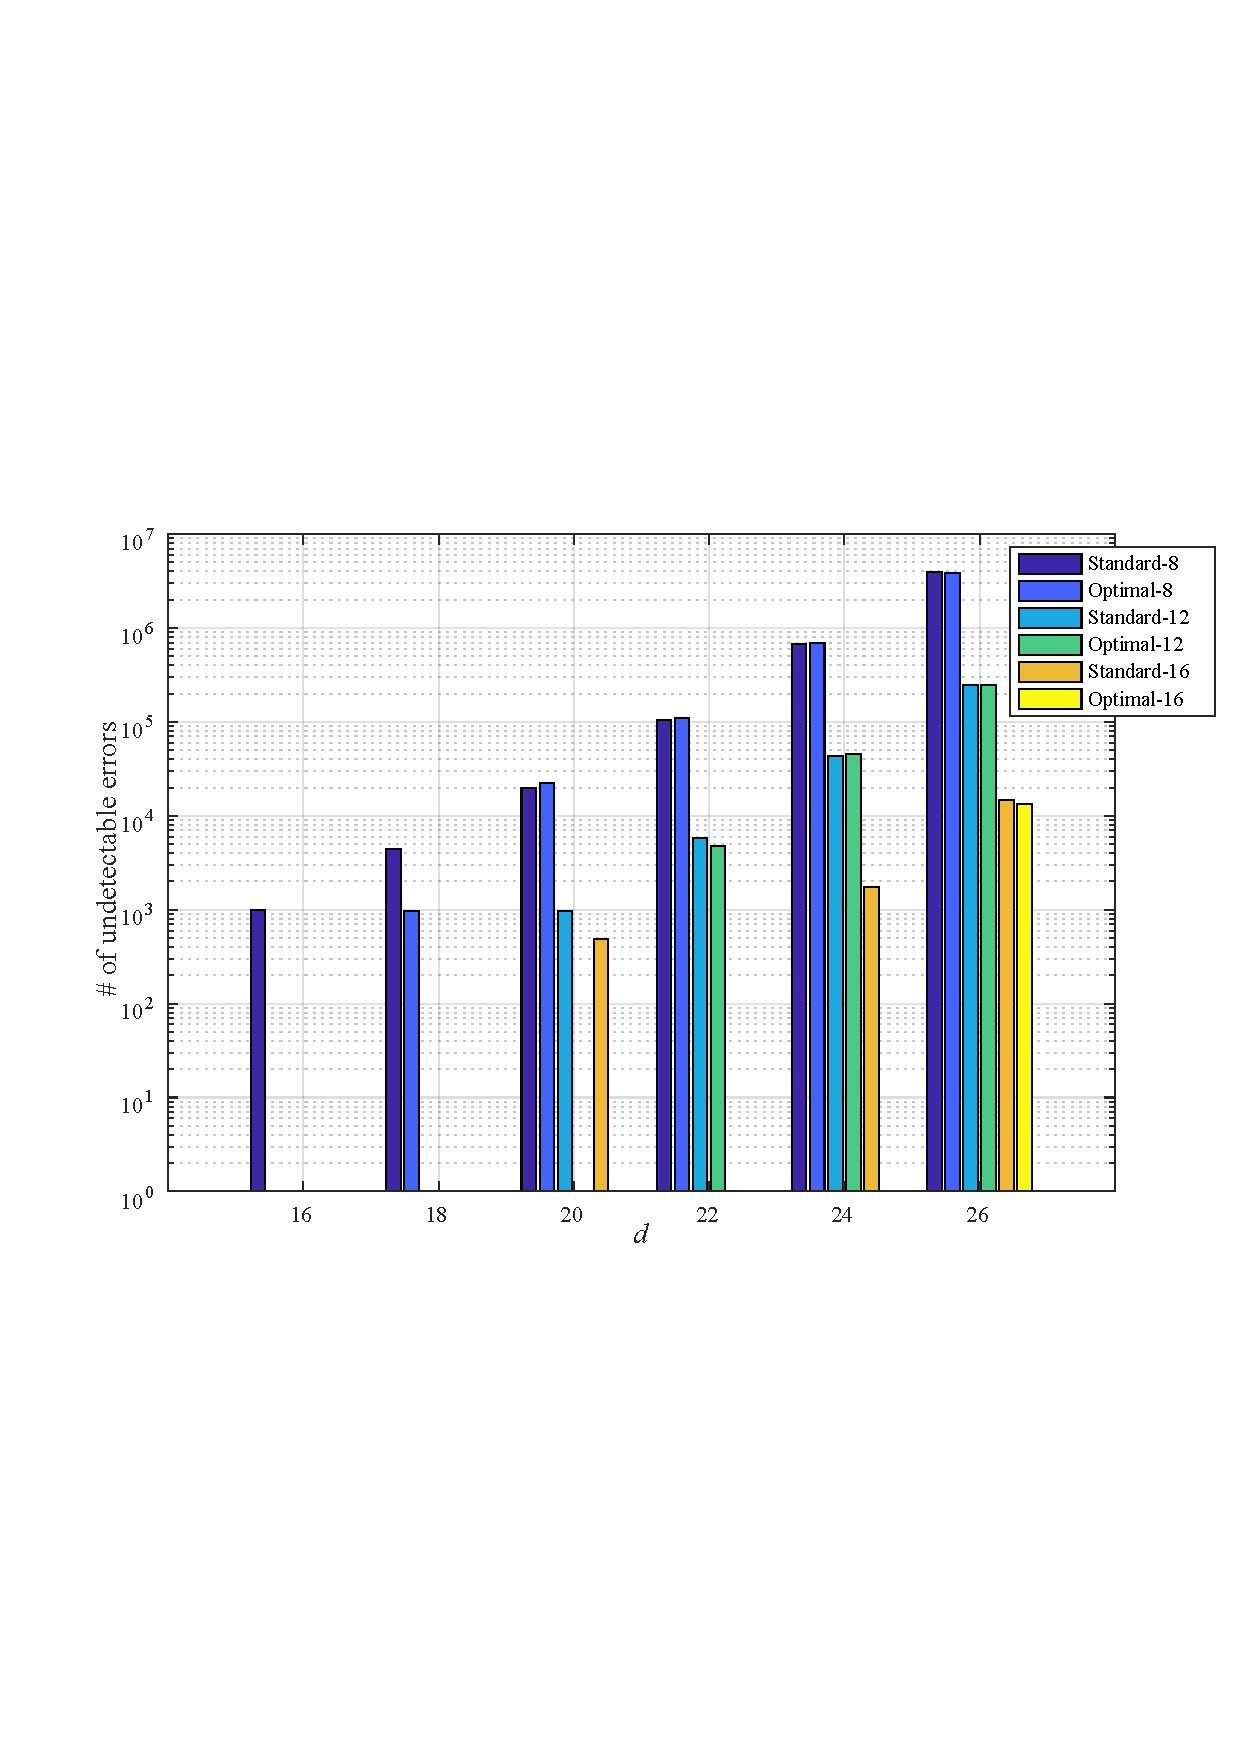
\includegraphics{Figures/spectrum_bar.pdf}}
% \caption{An example of figure insertion}
% \label{example_fig}
% \end{figure}

% \subsection{Equations}
% An example of equations is given as follows.
% \begin{theorem}
% Let $a$, $b$, $c$ denote the sides of a triangle, respectively. If $a\perp b$, the pythagoras theorem is given as follows.
% \begin{align}
% c^2 = a^2 + b^2
% \end{align}
% \end{theorem}

% \subsection{Tables}
% An example of tables is shown in Table \ref{example_table}.
% \renewcommand\arraystretch{1.1}
% \begin{table}[h]
% \center
% \caption{Standard CRC Codes versus Optimal CRC Codes for Convolutional Code $G=(561~753)$ with $n=504$ Bits}
% \scalebox{0.9}{
% \begin{tabular}{r|c|c|cccccc}
% \hline
% \multirow{2}{*}{Name} & \multirow{2}{*}{Gen. Poly.} & \multicolumn{7}{c}{Undetected Error Distance Spectrum} \\
% \cline{3-9}
%  & & $d$ & 16 & 18 & 20 & 22 & 24 & 26 \\\hline\hline
% Standard-8 & \multicolumn{1}{l}{0x19B} & & 983 & 4387 & 19909 & 105000 & 672724 & 3972970\\
% Optimal-8 & \multicolumn{1}{l}{0x19D} & & 0 & 979 & 22349 & 111304 & 686314 & 3830340\\\hline
% Standard-12 & \multicolumn{1}{l}{0x180F} & & 0 & 0 & 969 & 5815 & 42893 & 245211 \\
% Optimal-12 & \multicolumn{1}{l}{0x108B} & & 0 & 0 & 0 & 4793 & 45795 & 246729\\\hline
% Standard-16 & \multicolumn{1}{l}{0x11021} & & 0 & 0 & 484 & 0 & 1765 & 14752\\
% Optimal-16 & \multicolumn{1}{l}{0x1F8FD} & & 0 & 0 & 0 & 0 & 0 & 13240\\\hline
% \end{tabular}}
% \label{example_table}
% \end{table}


\section{Facebook network}

\subsection{Structural properties of the facebook network}

The facebook network is plotted in Fig. \ref{fig:facebook_network}.
\begin{figure}[h]
\centering
\scalebox{0.7}{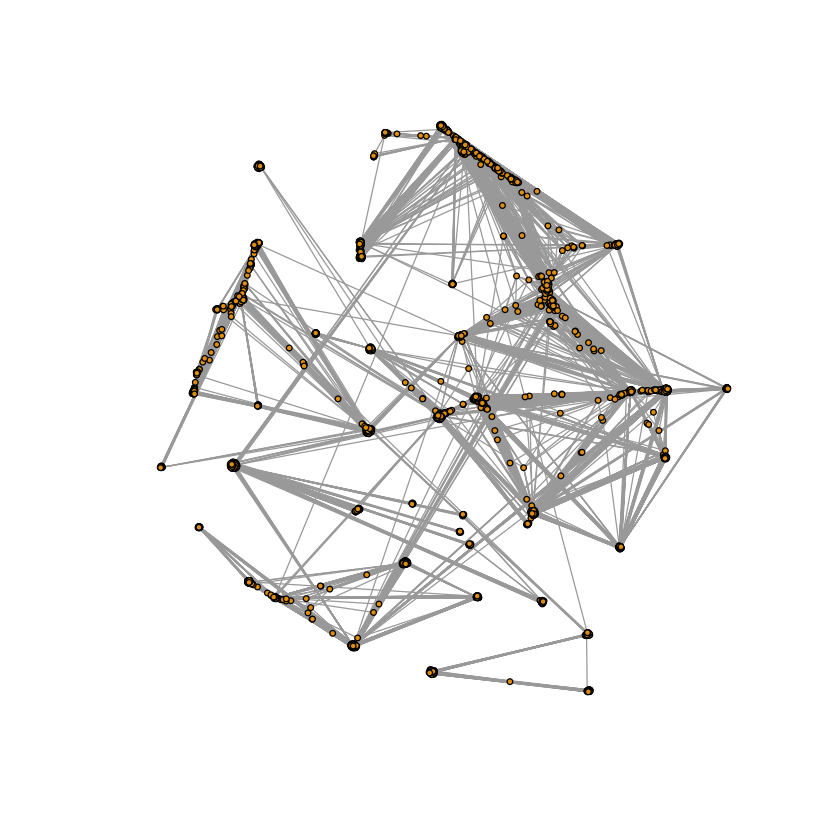
\includegraphics{Figures/hj_01}}
\caption{Facebook network}
\label{fig:facebook_network}
\end{figure}

\textcolor{red}{Question 1: Is the facebook network connected? If not, find the giant connected component (GCC) of the network and report the size of the GCC.}

The facebook network is connected.\\

\textcolor{red}{Question 2: Find the diameter of the network. If the network is not connected, then find the diameter of the GCC.}

The diameter of the Facebook network is $8$.\\

\textcolor{red}{Question 3: Plot the degree distribution of the facebook network and report the average degree.}

The degree distribution of the Facebook network is shown in Fig. \ref{fig:deg_distribution}. The average degree is $43.69101$.\\
\begin{figure}[t]
\centering
\scalebox{0.7}{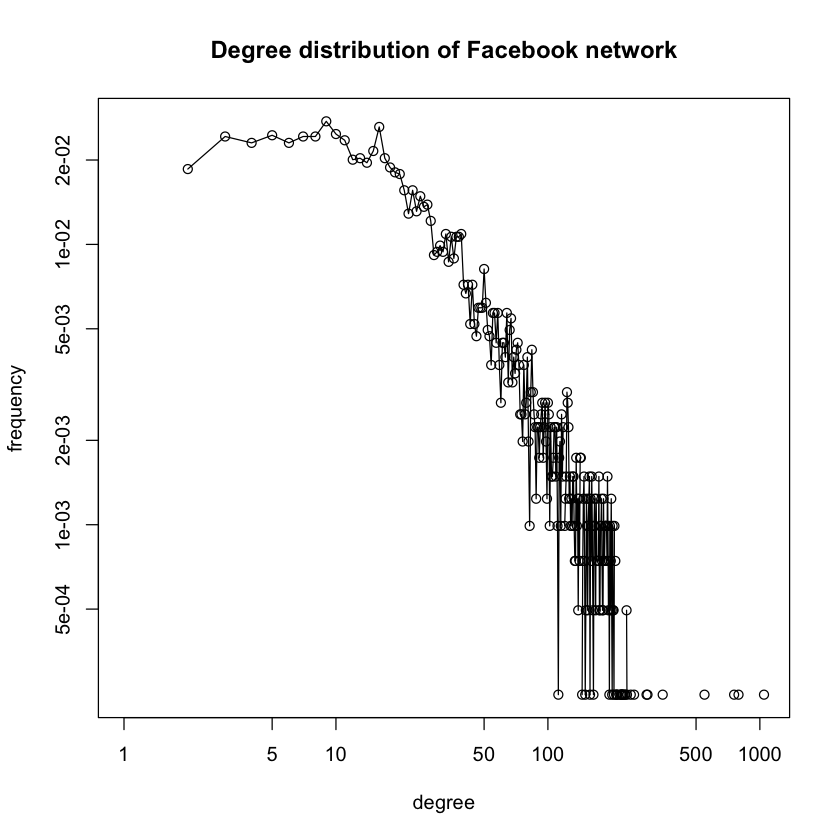
\includegraphics{Figures/hj_02}}
\caption{Degree distribution of the Facebook network}
\label{fig:deg_distribution}
\end{figure}

\textcolor{red}{Question 4: Plot the degree distribution of question 3 in a log-log scale. Try to fit a line to the plot and estimate the slope of the line.}

The degree distribution of Facebook network in log-log scale is shown in Fig. \ref{fig:deg_distribution_log}. In order to find a line which fits the data, we consider the data starting from $20$-th and ends $6$ before the end, thus, with linear regression analysis, the line we find is as follows.
\begin{align}
y=1.032-1.607x
\end{align}
where $y$ represents the $\log(frequency)$ and $x$ represents the $\log(degree)$. The estimated slope is $-1.607$.
\begin{figure}[t]
\centering
\scalebox{0.8}{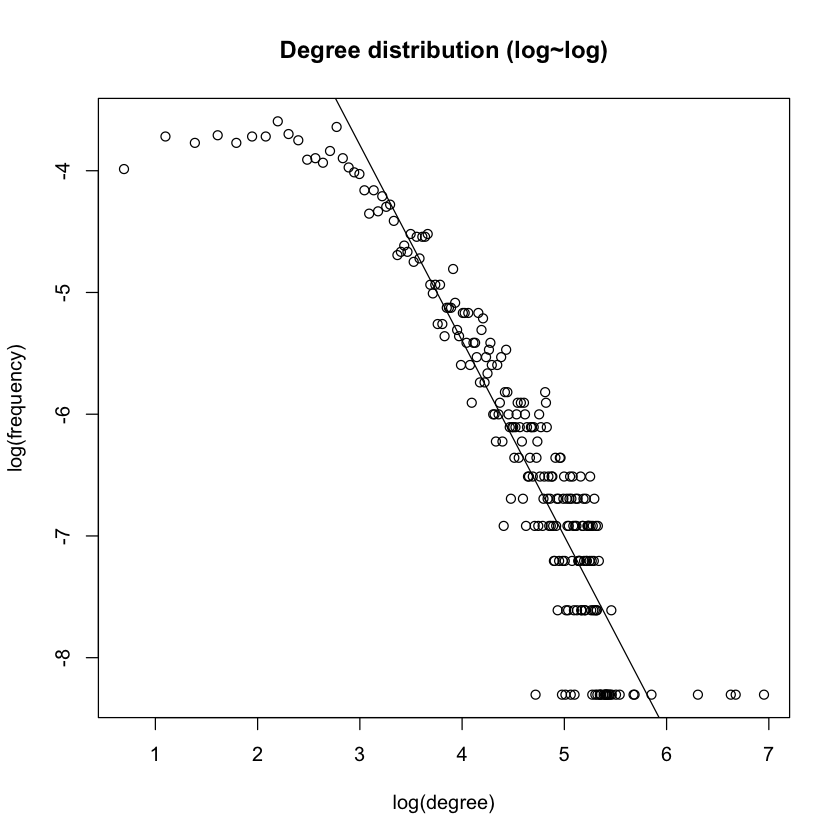
\includegraphics{Figures/hj_03}}
\caption{Degree distribution of the Facebook network in log-log scale}
\label{fig:deg_distribution_log}
\end{figure}

\subsection{Personalized network}
\textcolor{red}{Question 5: Create a personalized network of the user whose ID is 1. How many nodes and edges does this personalized network have?}

\begin{figure}[h]
\centering
\scalebox{0.7}{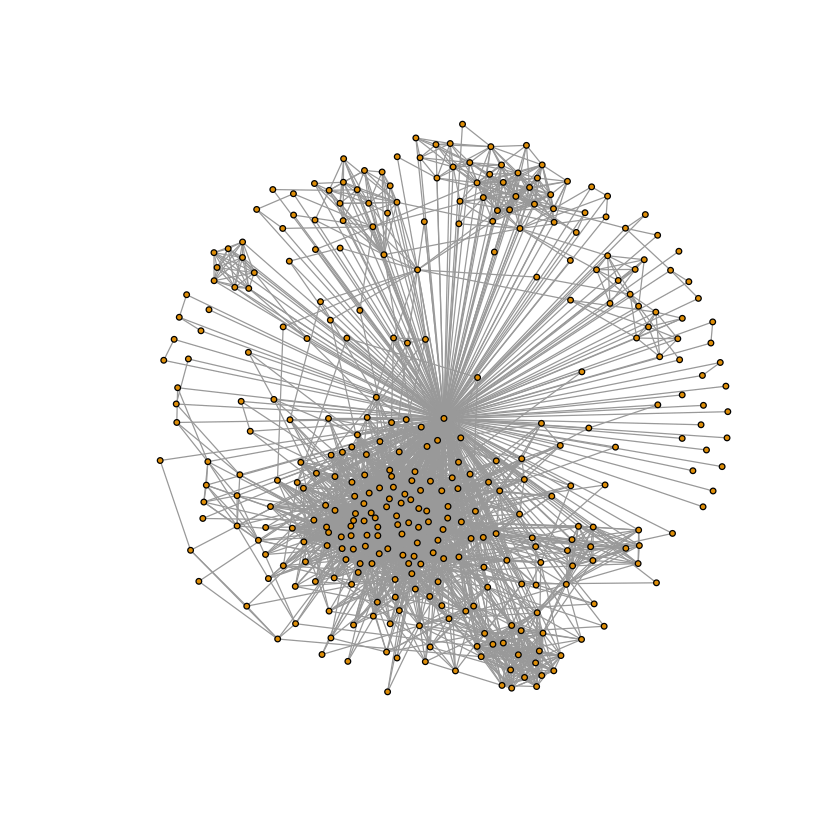
\includegraphics{Figures/hj_04}}
\caption{Personalized network of user with ID $1$}
\label{fig:personalized_net}
\end{figure}

The personalized network is shown in Fig. \ref{fig:personalized_net}. The number of nodes is $348$, and the number of edges is $2866$.\\

\textcolor{red}{Question 6: What is the diameter of the personalized network? Please state a trivial upper and lower bound for the diameter of the personalized network.}

The diameter of the personalized netowrk is $2$. A trivial upper bound of the diameter of the personalized network is $2$ and the lower bound of the personalized network is $1$.\\

\textcolor{red}{Question 7: In the context of the personalized network, what is the meaning of the diameter of the personalized network to be equal to the upper bound you derived in question 6. What is the meaning of the diameter
of the personalized network to be equal to the lower bound you derived in question 6?}

The meaning is that: given the core node of the personalized network, when the number of the neighbor nodes is $1$, clearly the diameter of this network is $1$; If the number of the neighbor nodes is greater than $1$, since all neighbor nodes are connected to the core node, thus the diameter of this network is $2$.


\subsection{Core node’s personalized network}

There are $40$ core nodes in the Facebook network, which is the nodes that have more than $200$ neighbors i.e. the degree of the nodes is greater than $200$. And the average degree of the core nodes is $279$.

\subsubsection{Community structure of core node’s personalized network}

We aim to find the community structure and compute the modularity scores using Fast-Greedy, Edge-Betweenness, and Infomap community detection algorithms for each of some core nodes’ personalized network.

For Node ID $1$, the community figures based on different algorithms are shown in Fig \ref{1_3_1_1}, Fig \ref{1_3_1_2} and Fig \ref{1_3_1_3}.

\begin{figure}
\centering
\begin{minipage}[t]{0.48\textwidth}
\centering
\scalebox{1}{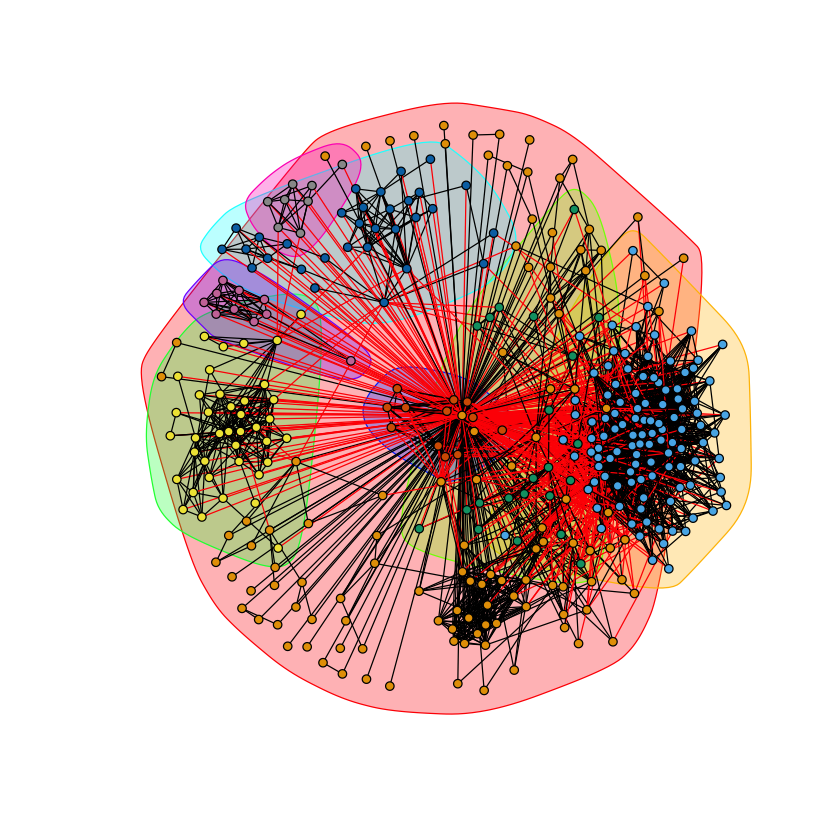
\includegraphics{Figures/1_3_1_1.png}}
\caption{community structure using Fast-Greedy algorithms}
\label{1_3_1_1}
\end{minipage}
\begin{minipage}[t]{0.48\textwidth}
\centering
\scalebox{1}{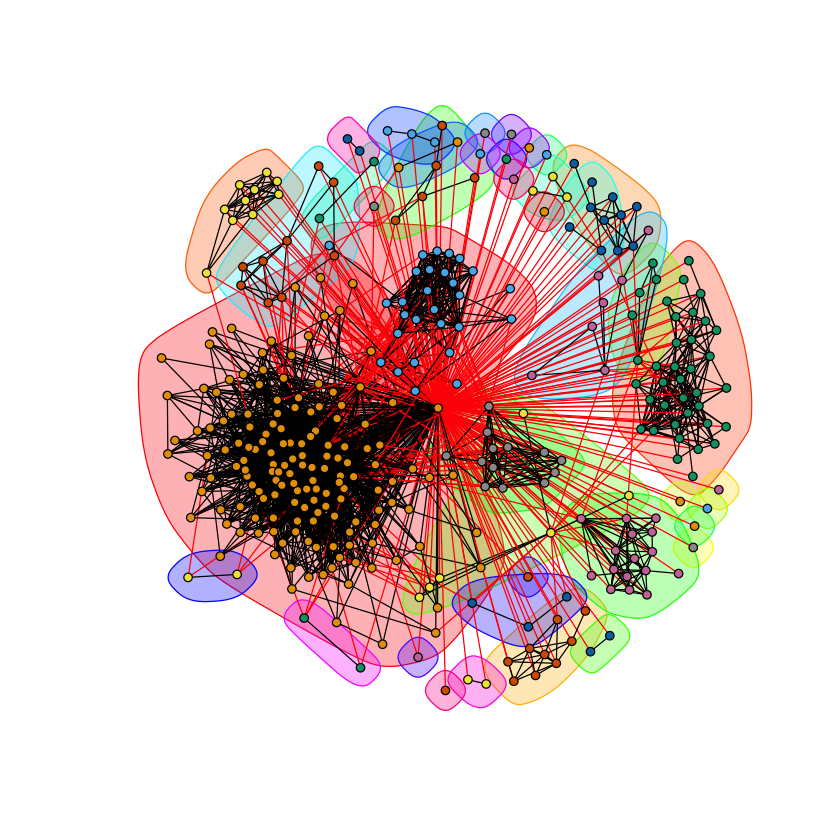
\includegraphics{Figures/1_3_1_2.png}}
\caption{community structure using Edge-Betweenness algorithms}
\label{1_3_1_2}
\end{minipage}
\end{figure}
\begin{figure}
\centering
\scalebox{0.5}{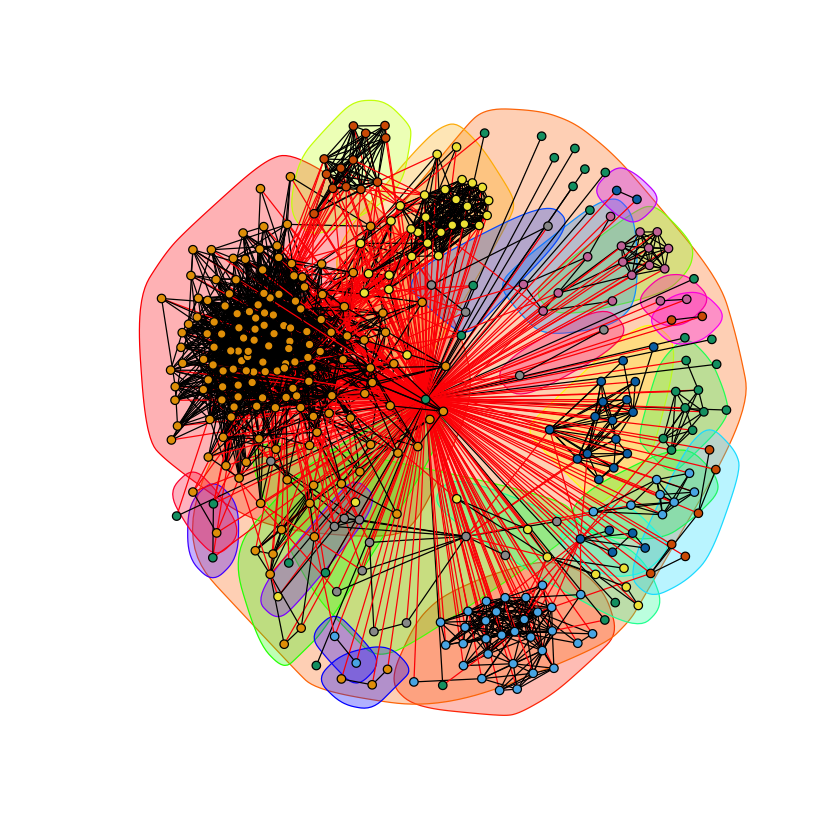
\includegraphics{Figures/1_3_1_3.png}}
\caption{community structure using Infomap algorithms}
\label{1_3_1_3}
\end{figure}


For Node ID $108$, the community figures based on different algorithms are shown in Fig \ref{1_3_1_4}, Fig \ref{1_3_1_5} and Fig \ref{1_3_1_6}.

\begin{figure}
\centering
\begin{minipage}[t]{0.48\textwidth}
\centering
\scalebox{1}{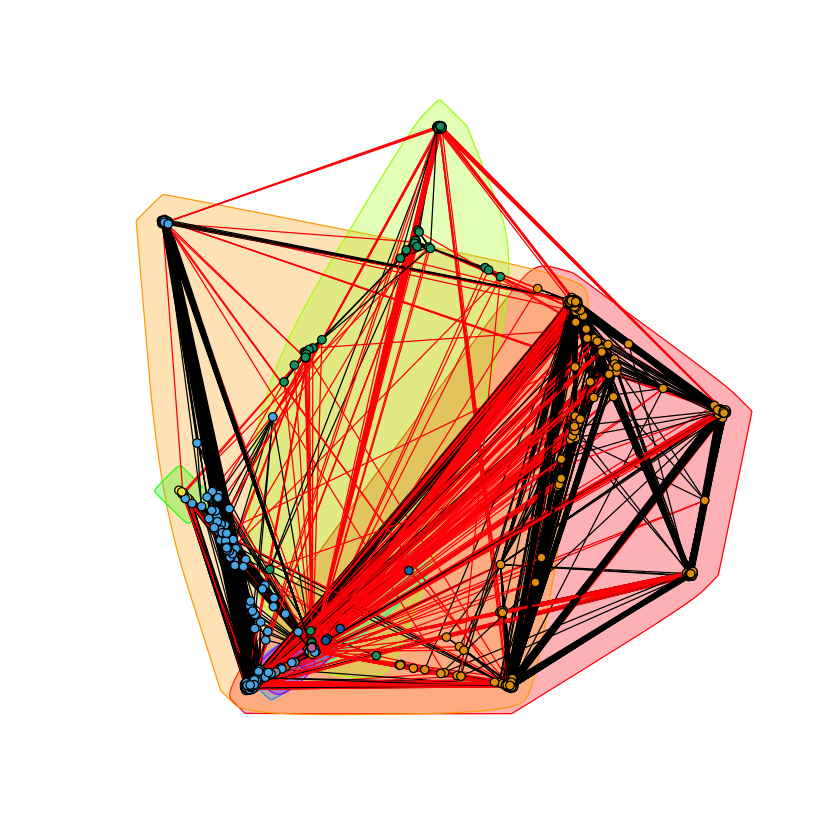
\includegraphics{Figures/1_3_1_4.png}}
\caption{community structure using Fast-Greedy algorithms}
\label{1_3_1_4}
\end{minipage}
\begin{minipage}[t]{0.48\textwidth}
\centering
\scalebox{1}{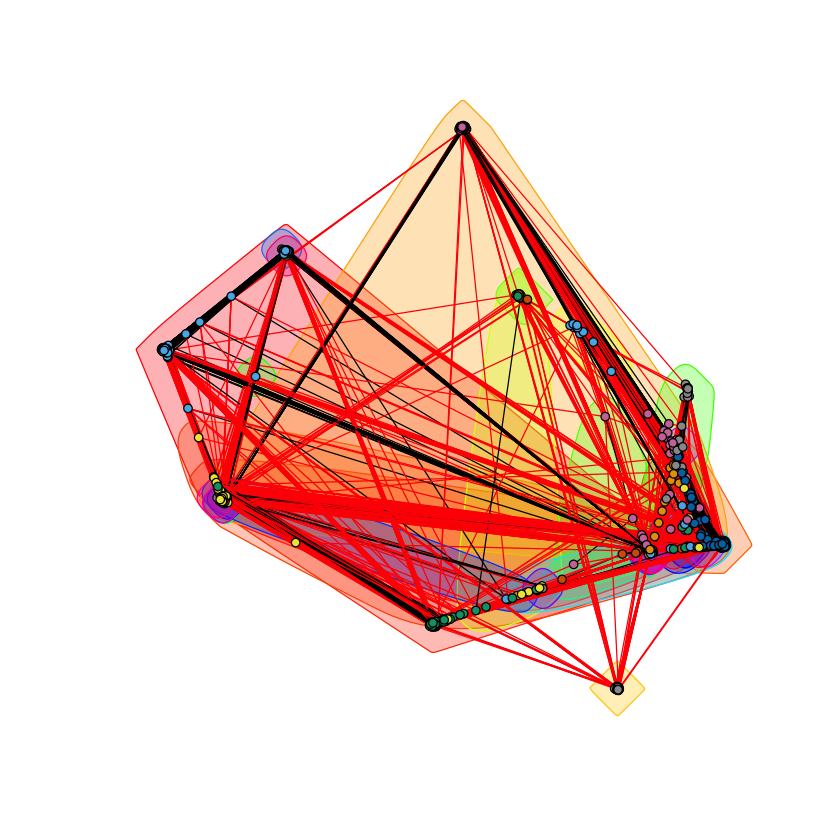
\includegraphics{Figures/1_3_1_5.png}}
\caption{community structure using Edge-Betweenness algorithms}
\label{1_3_1_5}
\end{minipage}
\end{figure}
\begin{figure}
\centering
\scalebox{0.5}{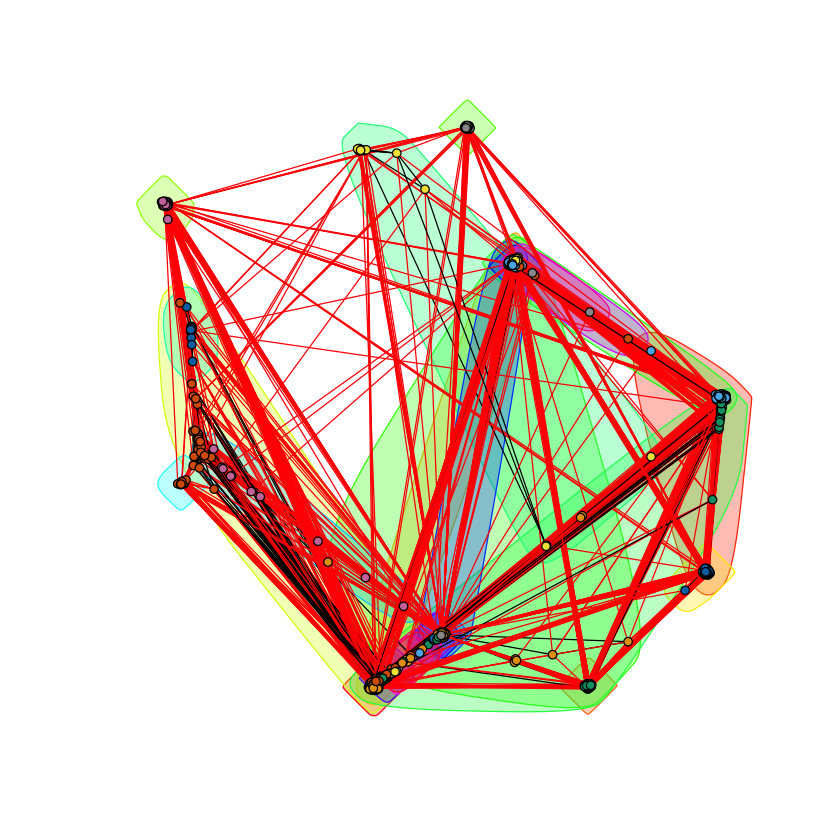
\includegraphics{Figures/1_3_1_6.png}}
\caption{community structure using Infomap algorithms}
\label{1_3_1_6}
\end{figure}

For Node ID $349$, the community figures based on different algorithms are shown in Fig \ref{1_3_1_7}, Fig \ref{1_3_1_8} and Fig \ref{1_3_1_9}.

\begin{figure}
\centering
\begin{minipage}[t]{0.48\textwidth}
\centering
\scalebox{1}{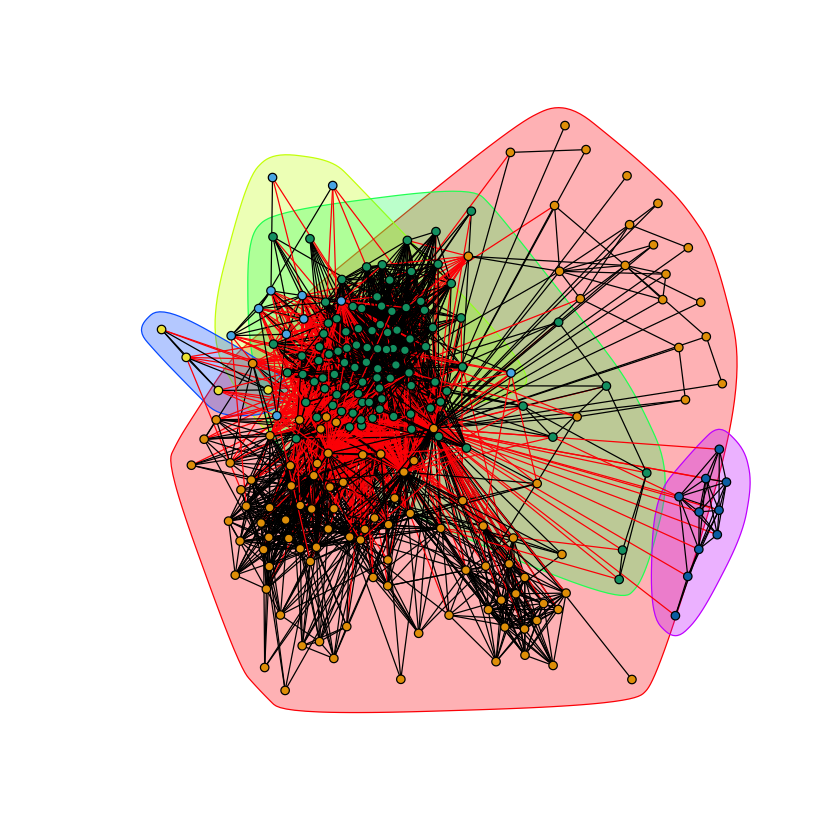
\includegraphics{Figures/1_3_1_7.png}}
\caption{community structure using Fast-Greedy algorithms}
\label{1_3_1_7}
\end{minipage}
\begin{minipage}[t]{0.48\textwidth}
\centering
\scalebox{1}{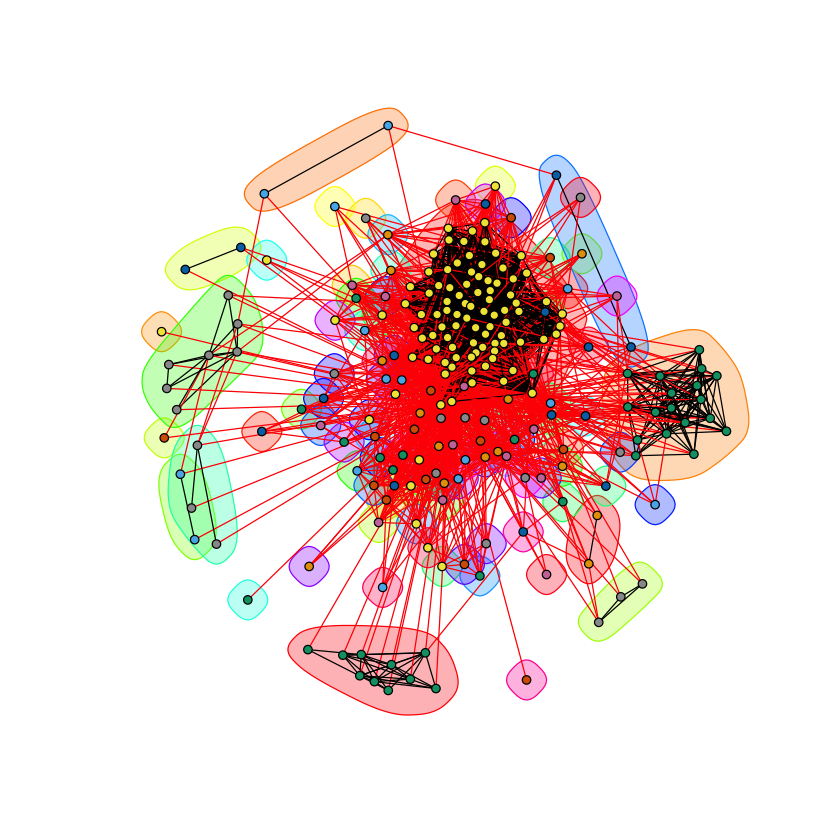
\includegraphics{Figures/1_3_1_8.png}}
\caption{community structure using Edge-Betweenness algorithms}
\label{1_3_1_8}
\end{minipage}
\end{figure}
\begin{figure}
\centering
\scalebox{0.5}{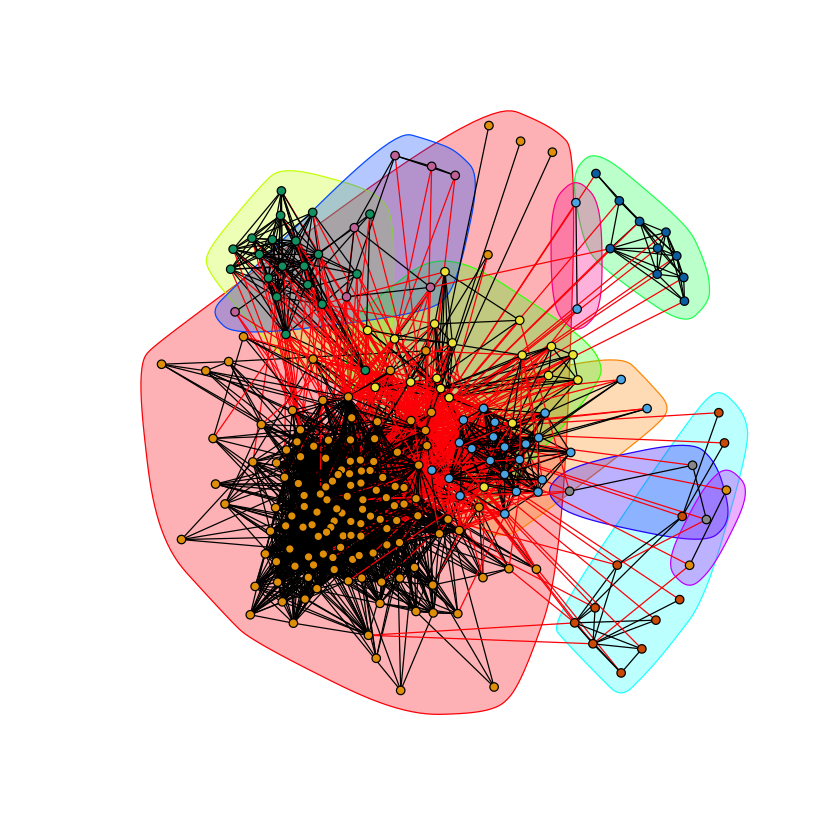
\includegraphics{Figures/1_3_1_9.png}}
\caption{community structure using Infomap algorithms}
\label{1_3_1_9}
\end{figure}

For Node ID $484$, the community figures based on different algorithms are shown in Fig \ref{1_3_1_10}, Fig \ref{1_3_1_11} and Fig \ref{1_3_1_12}.

\begin{figure}
\centering
\begin{minipage}[t]{0.48\textwidth}
\centering
\scalebox{1}{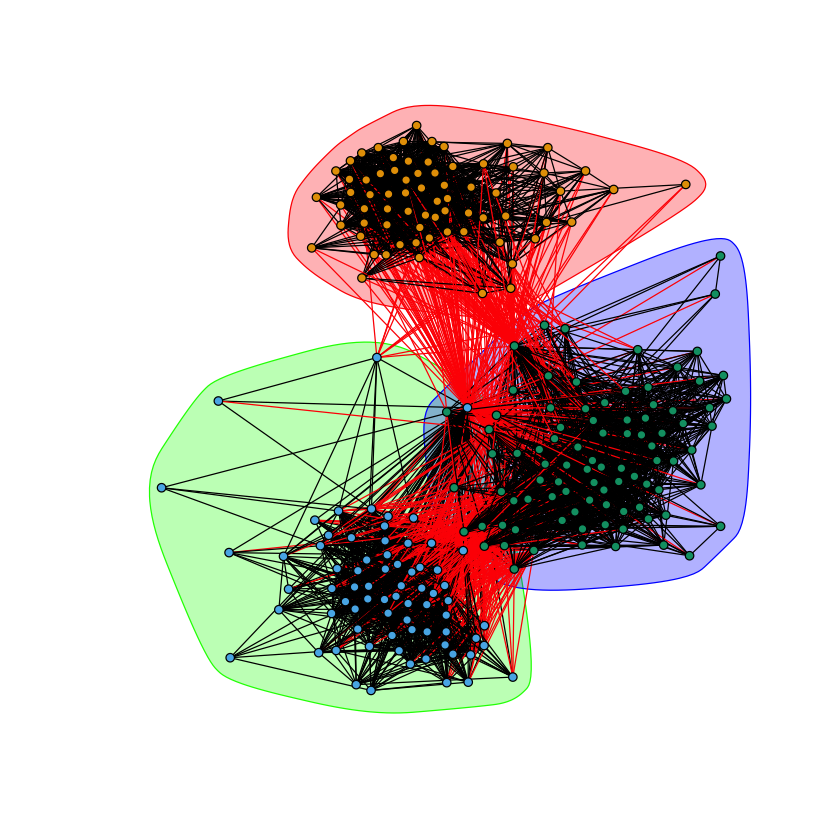
\includegraphics{Figures/1_3_1_10.png}}
\caption{community structure using Fast-Greedy algorithms}
\label{1_3_1_10}
\end{minipage}
\begin{minipage}[t]{0.48\textwidth}
\centering
\scalebox{1}{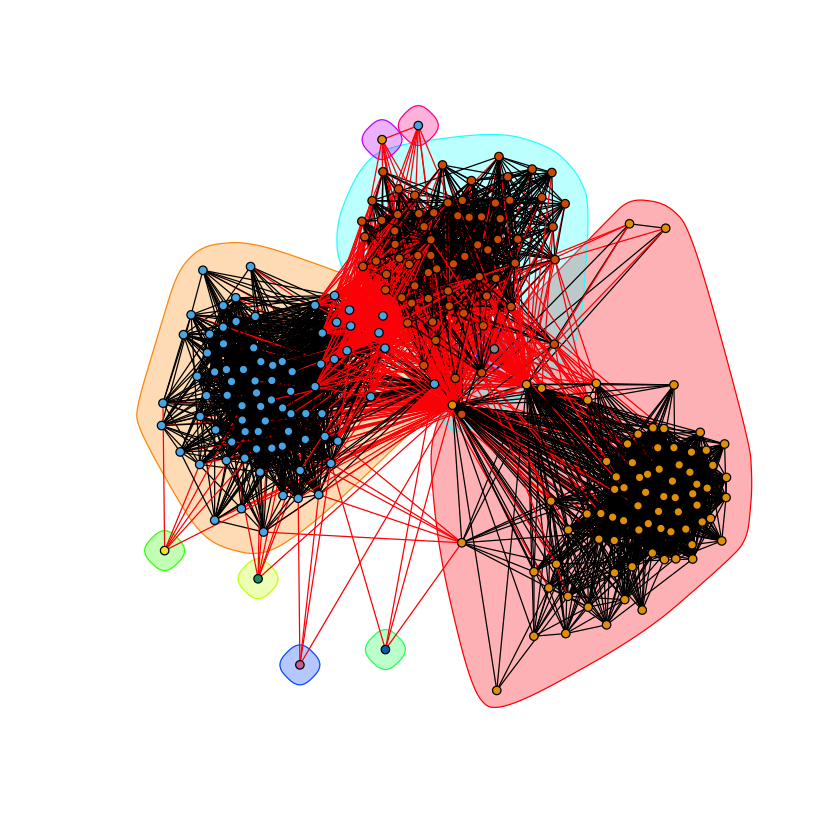
\includegraphics{Figures/1_3_1_11.png}}
\caption{community structure using Edge-Betweenness algorithms}
\label{1_3_1_11}
\end{minipage}
\end{figure}
\begin{figure}
\centering
\scalebox{0.5}{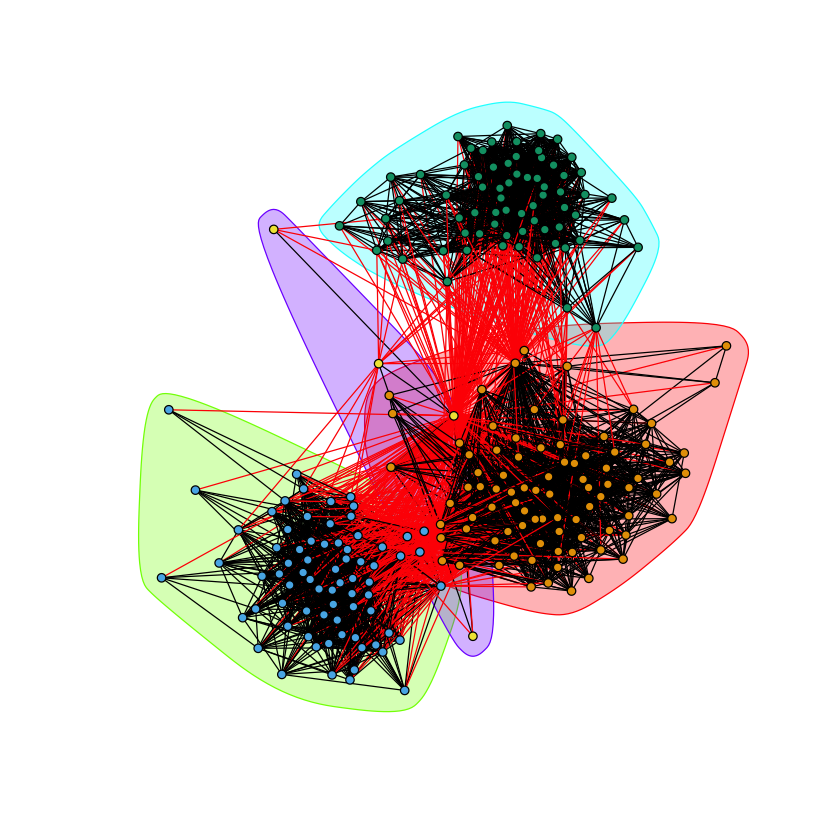
\includegraphics{Figures/1_3_1_12.png}}
\caption{community structure using Infomap algorithms}
\label{1_3_1_12}
\end{figure}

For Node ID $1087$, the community figures based on different algorithms are shown in Fig \ref{1_3_1_13}, Fig \ref{1_3_1_14} and Fig \ref{1_3_1_15}.

\begin{figure}
\centering
\begin{minipage}[t]{0.48\textwidth}
\centering
\scalebox{1}{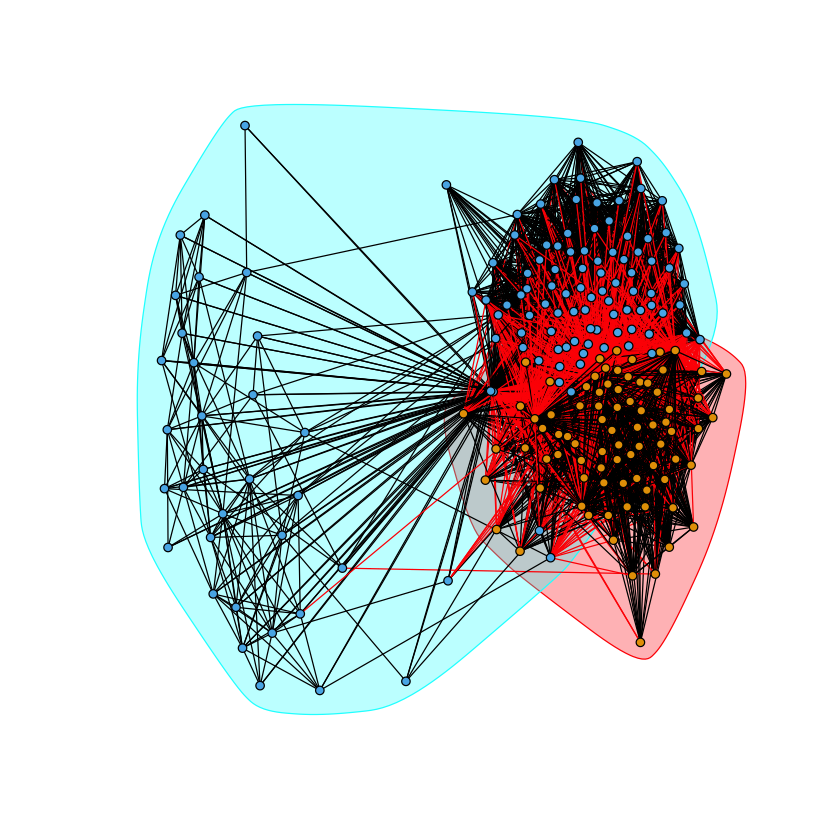
\includegraphics{Figures/1_3_1_13.png}}
\caption{community structure using Fast-Greedy algorithms}
\label{1_3_1_13}
\end{minipage}
\begin{minipage}[t]{0.48\textwidth}
\centering
\scalebox{1}{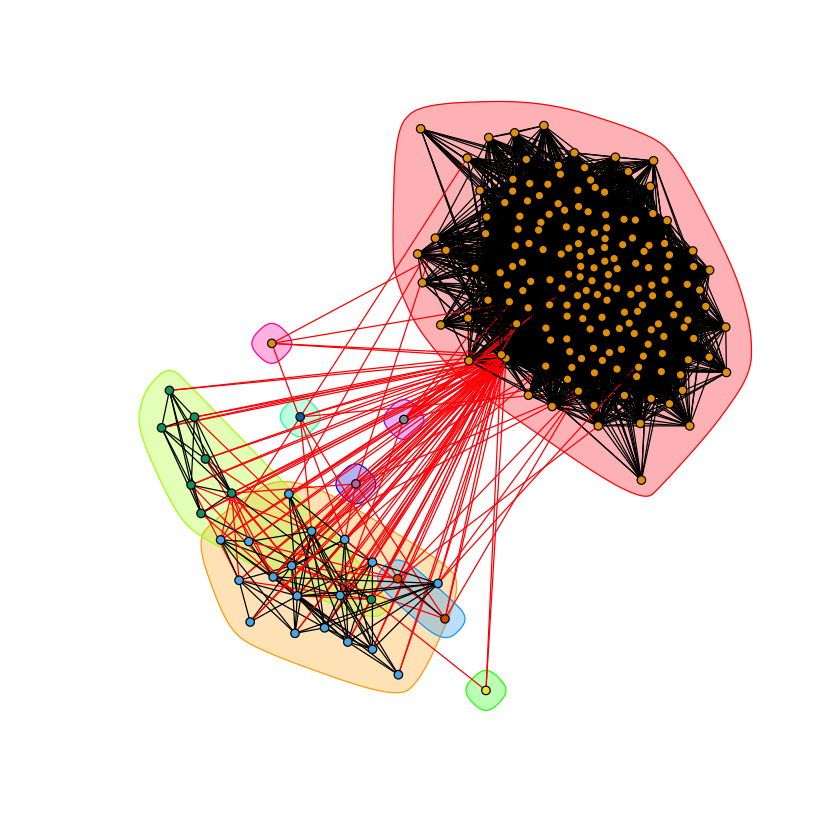
\includegraphics{Figures/1_3_1_14.png}}
\caption{community structure using Edge-Betweenness algorithms}
\label{1_3_1_14}
\end{minipage}
\end{figure}
\begin{figure}
\centering
\scalebox{0.5}{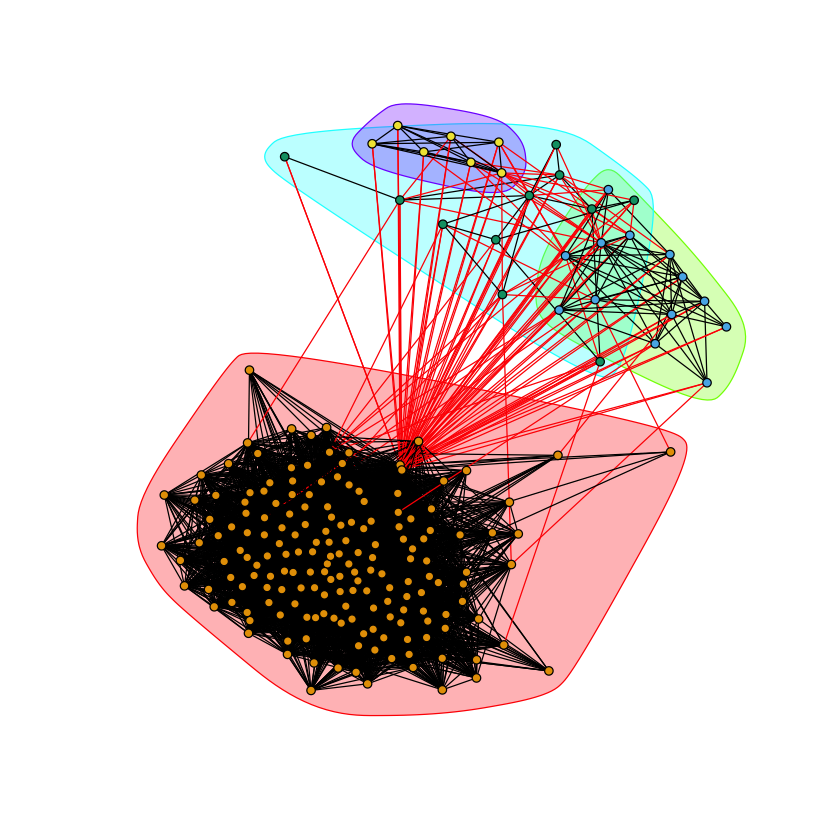
\includegraphics{Figures/1_3_1_15.png}}
\caption{community structure using Infomap algorithms}
\label{1_3_1_15}
\end{figure}

What's more, all the modularity scores from above core nodes' personalized network computed by different algorithms is shown in Table \ref{modtable}.

\begin{table}[h]
\center
\caption{The modularity scores for core nodes' personalized network}
\begin{tabular}{c|l|l|l} 
\textbf{Node ID} & \textbf{Fast-Greedy} & \textbf{Edge-Betweenness} & \textbf{Infomap}\\\hline
$1$ & $0.41310$ & $0.35330$ & $0.38912$\\
$108$ & $0.43592$ & $0.50675$ & $0.50842$\\
$349$ & $0.25171$ & $0.13352$ & $0.20375$\\
$484$ & $0.50700$ & $0.48909$ & $0.51527$\\
$1087$ & $0.14553$ & $0.02762$ & $0.02690$\\
\end{tabular}
\label{modtable}
\end{table}

Fast-greedy is very simple hierarchical approach, which is a bottom-up algorithm. It can achieve the goal of optimizing modularity in a greedy manner. This algorithm starts with a state that we treat every single node as a separate community, and communities are merged iteratively such that each merge yields the largest increase of the modularity value until the value would not increase any more. From the result we drew, we can see that this algorithm is pretty fast but extremely not accurate. There is no doubt that it is very common that a greedy method could suck in a local optimal and hardly find global optimal.

In comparison to Fast-greedy algorithm, edge-betweenness is also a hierarchical process but top-down. In this algorithm, network's edges are removed in the decreasing order of the number of shortest paths. The good thing is that this method yields good results since the edges connecting different communities are likely to be contained in multiple shortest paths, which makes this method very effective intuitively. Unfortunately, just like there is no perfect thing in the world, this algorithm is super time-consuming due to the computational complexity. Especially for node $108$'s personalized network, it took more than one hour to detect communities by this algorithm.

At last, Infomap algorithm is a method minimizing a random walker’s expected trajectory based on ideas of information theory. The Infomap method seems to be slightly better at detecting communities than fast-greedy and faster than edge-betweenness. It seems like Infomap is a kind of algorithm that we use when we don't want to wait for a very long time to compute for a large scale network but still want a satisfied result.

\subsubsection{Community structure with the core node removed}

In this part, we aim to explore the effect on the community structure of a core node’s personalized network when the core node itself is removed from the personalized network.

For Node ID $1$, the community figures based on different algorithms are shown in Fig \ref{1_3_2_1}, Fig \ref{1_3_2_2} and Fig \ref{1_3_2_3}.

\begin{figure}
\centering
\begin{minipage}[t]{0.48\textwidth}
\centering
\scalebox{1}{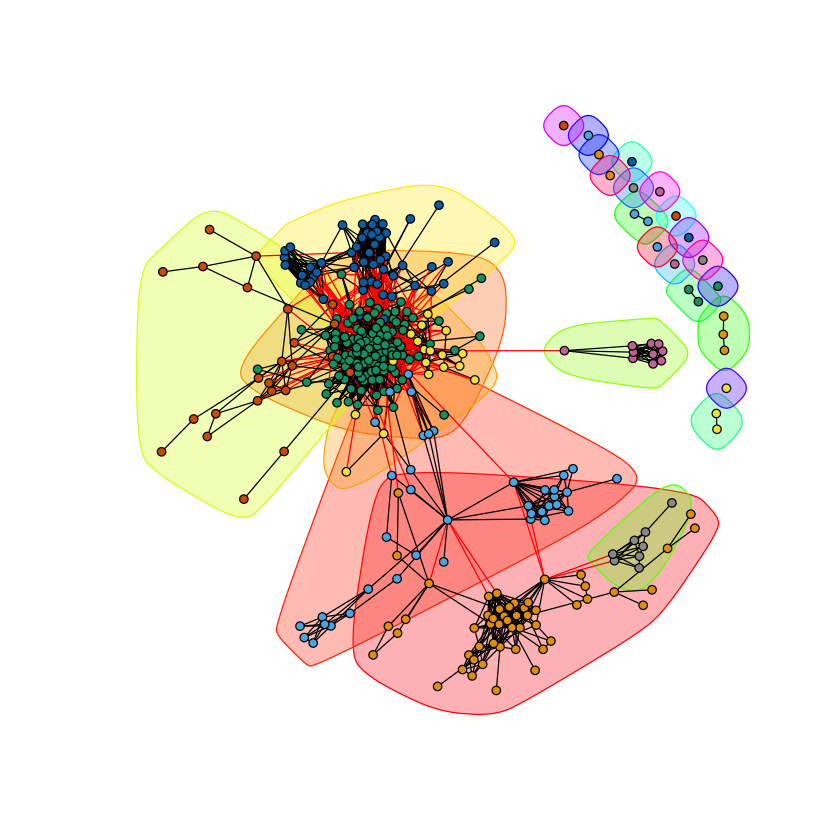
\includegraphics{Figures/1_3_2_1.png}}
\caption{community structure using Fast-Greedy algorithms}
\label{1_3_2_1}
\end{minipage}
\begin{minipage}[t]{0.48\textwidth}
\centering
\scalebox{1}{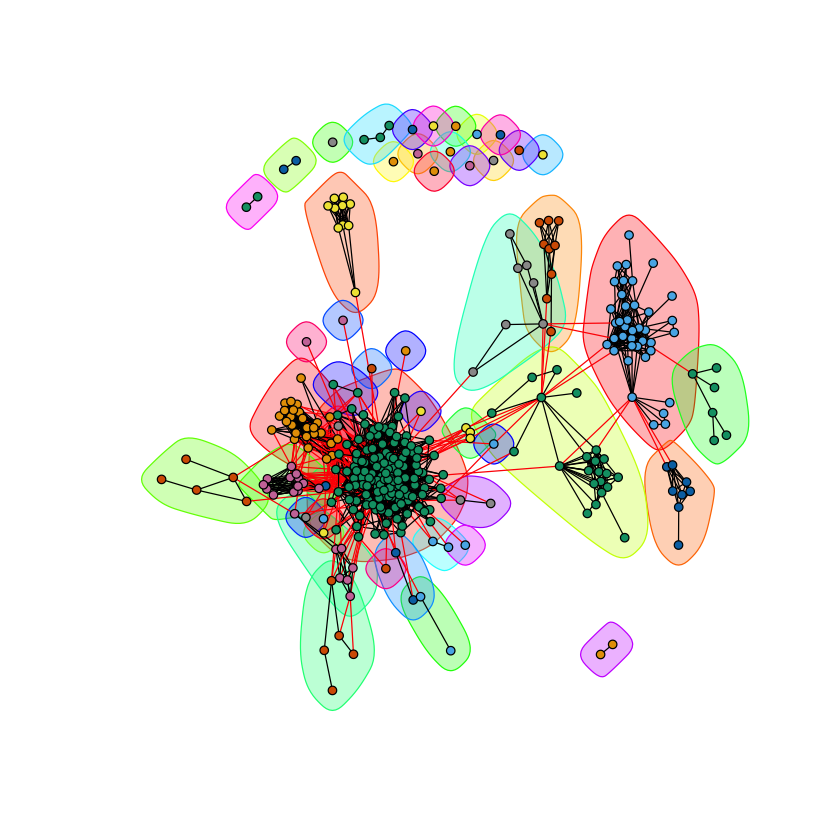
\includegraphics{Figures/1_3_2_2.png}}
\caption{community structure using Edge-Betweenness algorithms}
\label{1_3_2_2}
\end{minipage}
\end{figure}
\begin{figure}
\centering
\scalebox{0.5}{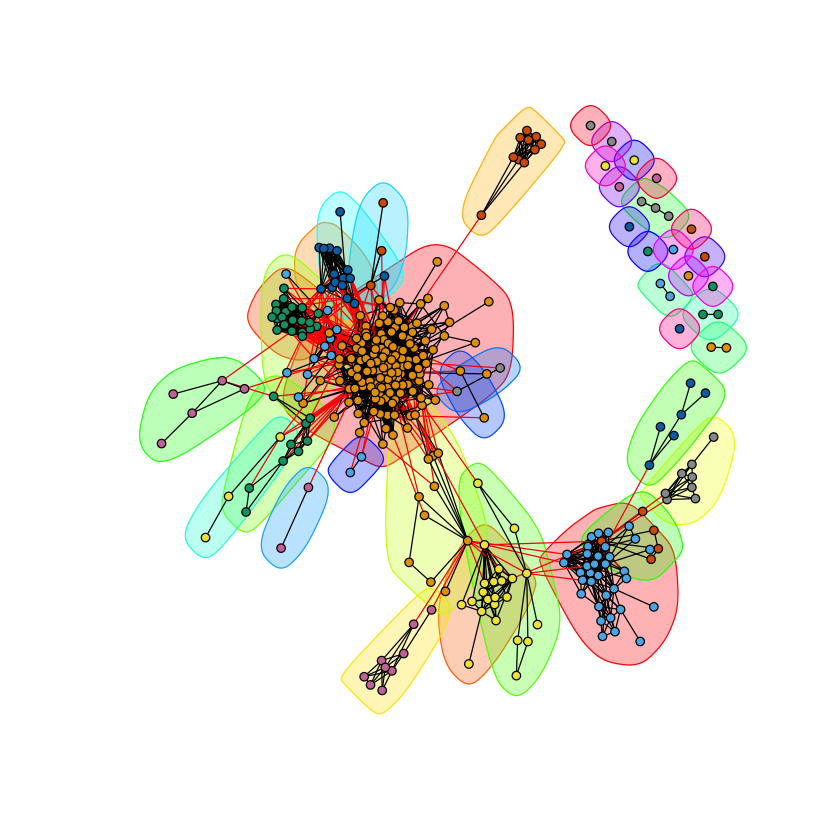
\includegraphics{Figures/1_3_2_3.png}}
\caption{community structure using Infomap algorithms}
\label{1_3_2_3}
\end{figure}

For Node ID $108$, the community figures based on different algorithms are shown in Fig \ref{1_3_2_4}, Fig \ref{1_3_2_5} and Fig \ref{1_3_2_6}.

\begin{figure}
\centering
\begin{minipage}[t]{0.48\textwidth}
\centering
\scalebox{1}{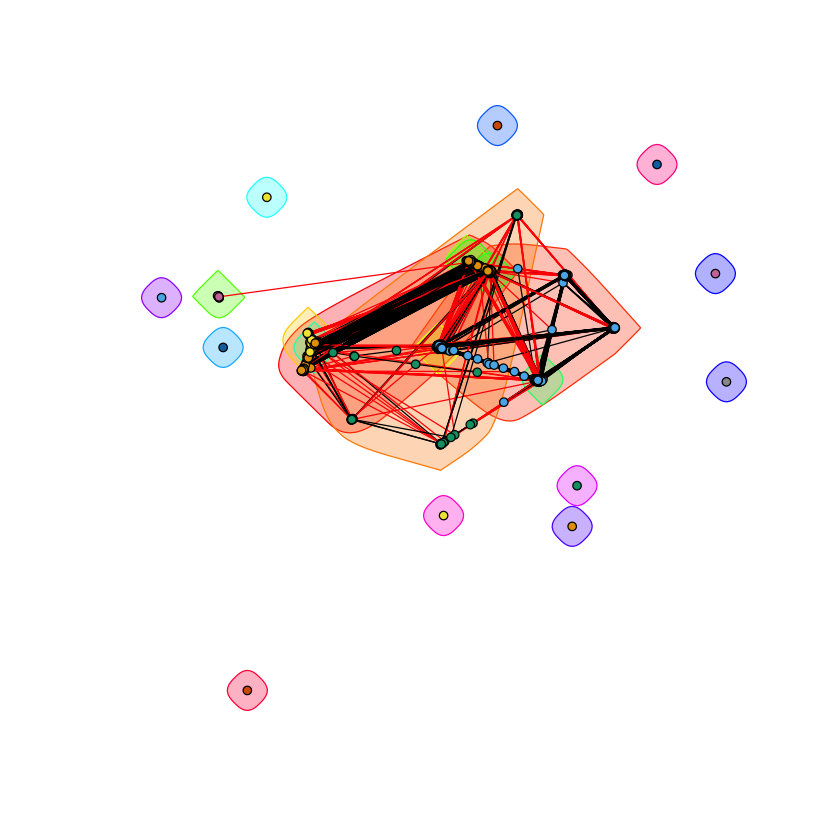
\includegraphics{Figures/1_3_2_4.png}}
\caption{community structure using Fast-Greedy algorithms}
\label{1_3_2_4}
\end{minipage}
\begin{minipage}[t]{0.48\textwidth}
\centering
\scalebox{1}{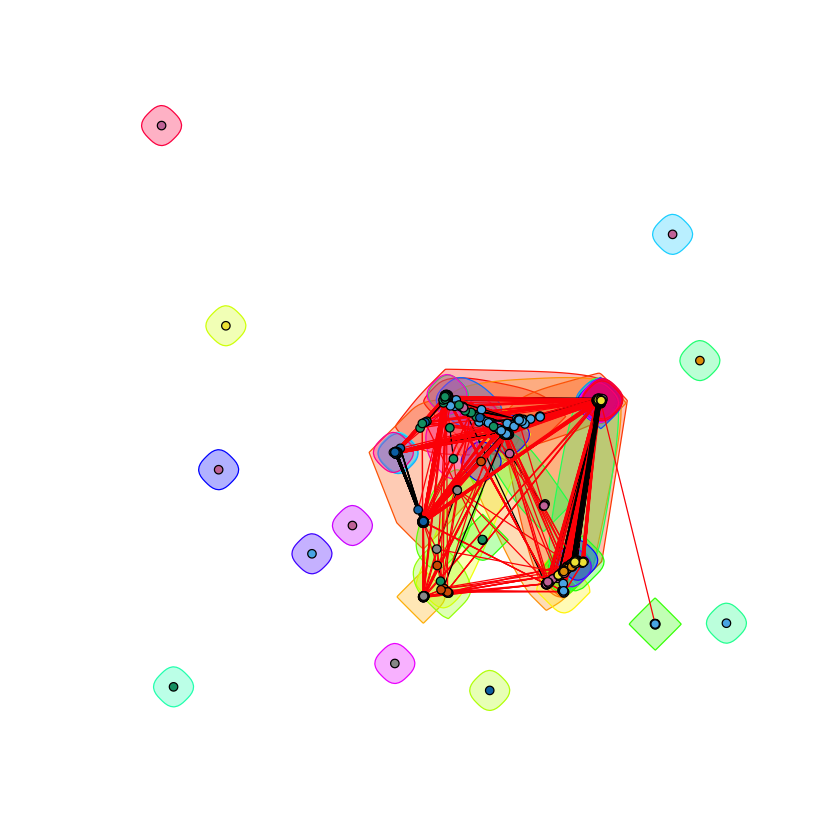
\includegraphics{Figures/1_3_2_5.png}}
\caption{community structure using Edge-Betweenness algorithms}
\label{1_3_2_5}
\end{minipage}
\end{figure}
\begin{figure}
\centering
\scalebox{0.5}{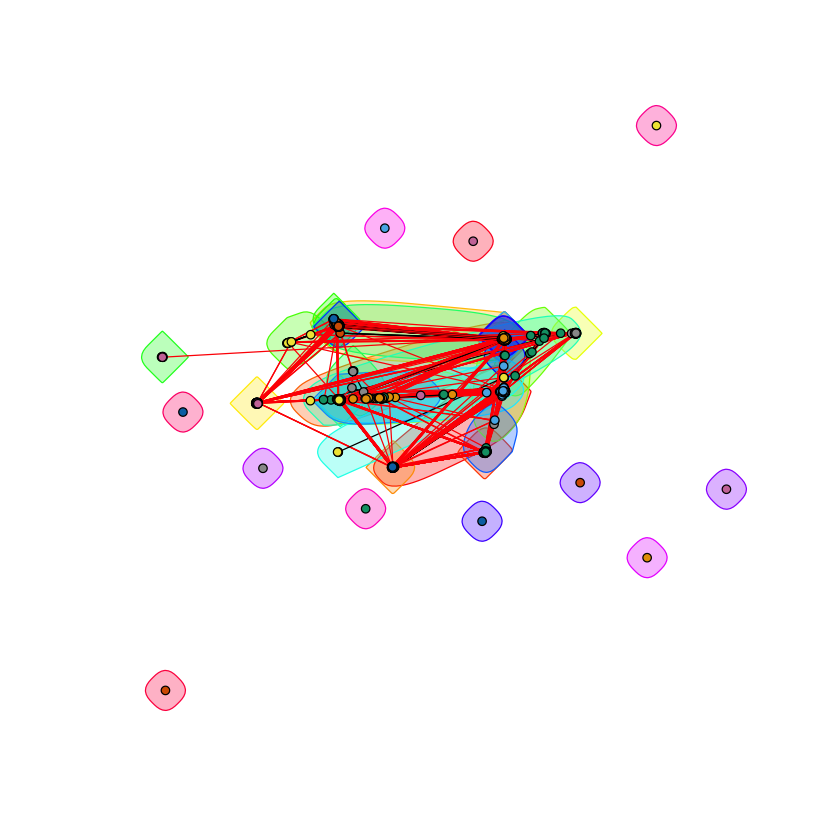
\includegraphics{Figures/1_3_2_6.png}}
\caption{community structure using Infomap algorithms}
\label{1_3_2_6}
\end{figure}

For Node ID $349$, the community figures based on different algorithms are shown in Fig \ref{1_3_2_7}, Fig \ref{1_3_2_8} and Fig \ref{1_3_2_9}.

\begin{figure}
\centering
\begin{minipage}[t]{0.48\textwidth}
\centering
\scalebox{1}{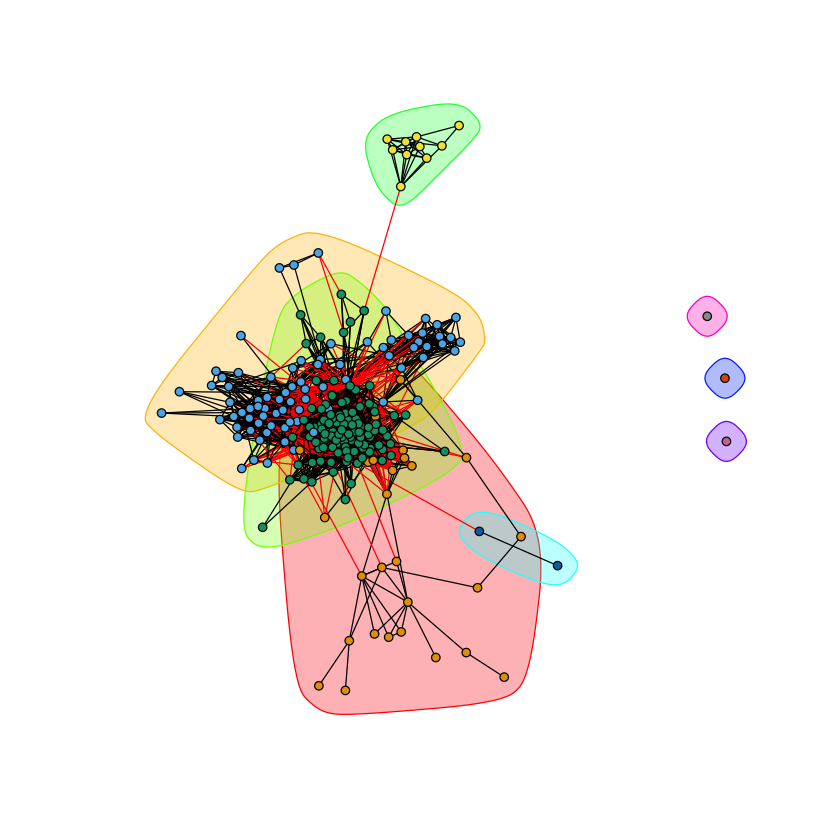
\includegraphics{Figures/1_3_2_7.png}}
\caption{community structure using Fast-Greedy algorithms}
\label{1_3_2_7}
\end{minipage}
\begin{minipage}[t]{0.48\textwidth}
\centering
\scalebox{1}{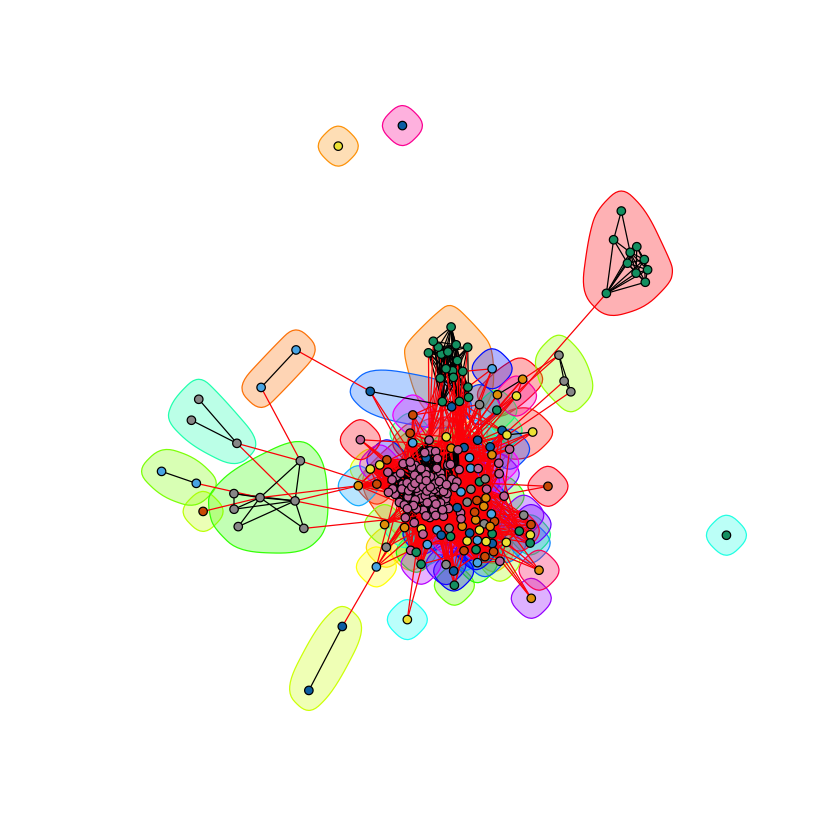
\includegraphics{Figures/1_3_2_8.png}}
\caption{community structure using Edge-Betweenness algorithms}
\label{1_3_2_8}
\end{minipage}
\end{figure}
\begin{figure}
\centering
\scalebox{0.5}{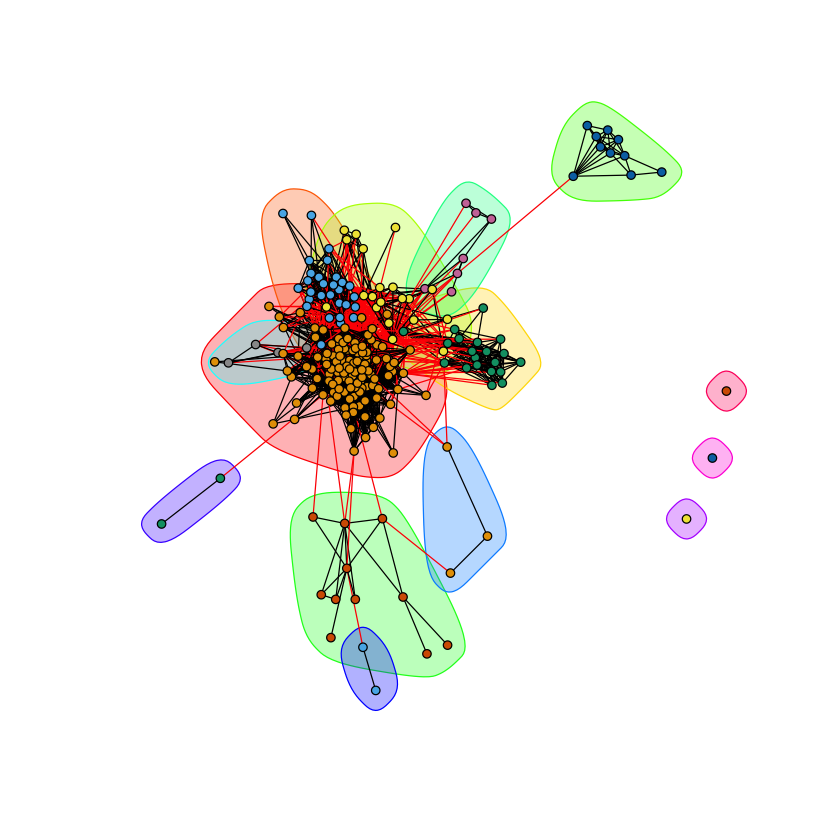
\includegraphics{Figures/1_3_2_9.png}}
\caption{community structure using Infomap algorithms}
\label{1_3_2_9}
\end{figure}

For Node ID $484$, the community figures based on different algorithms are shown in Fig \ref{1_3_2_10}, Fig \ref{1_3_2_11} and Fig \ref{1_3_2_12}.

\begin{figure}
\centering
\begin{minipage}[t]{0.48\textwidth}
\centering
\scalebox{1}{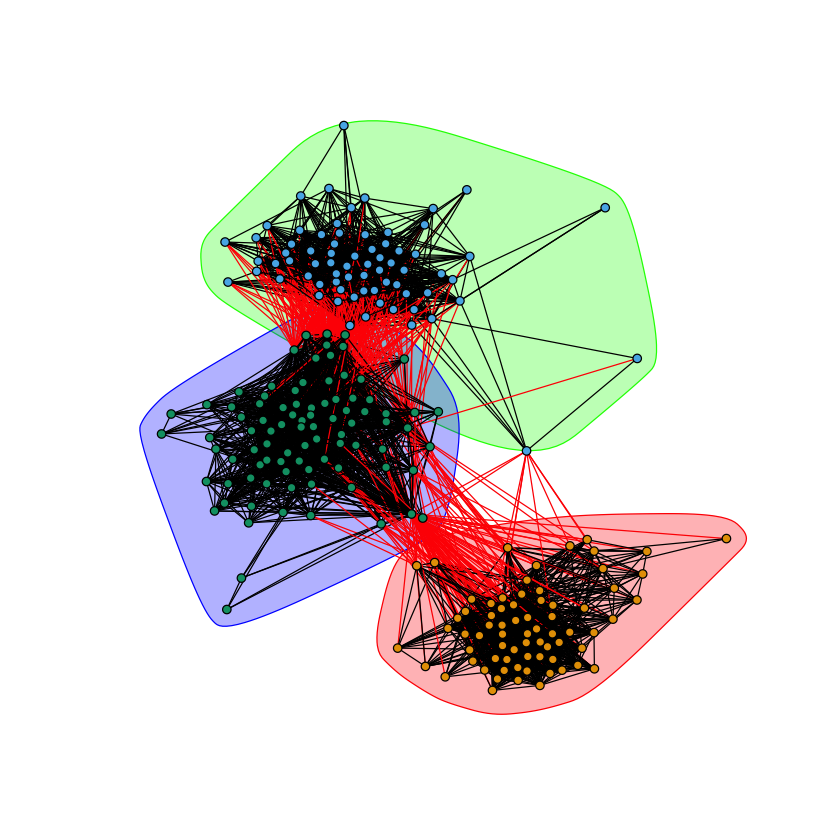
\includegraphics{Figures/1_3_2_10.png}}
\caption{community structure using Fast-Greedy algorithms}
\label{1_3_2_10}
\end{minipage}
\begin{minipage}[t]{0.48\textwidth}
\centering
\scalebox{1}{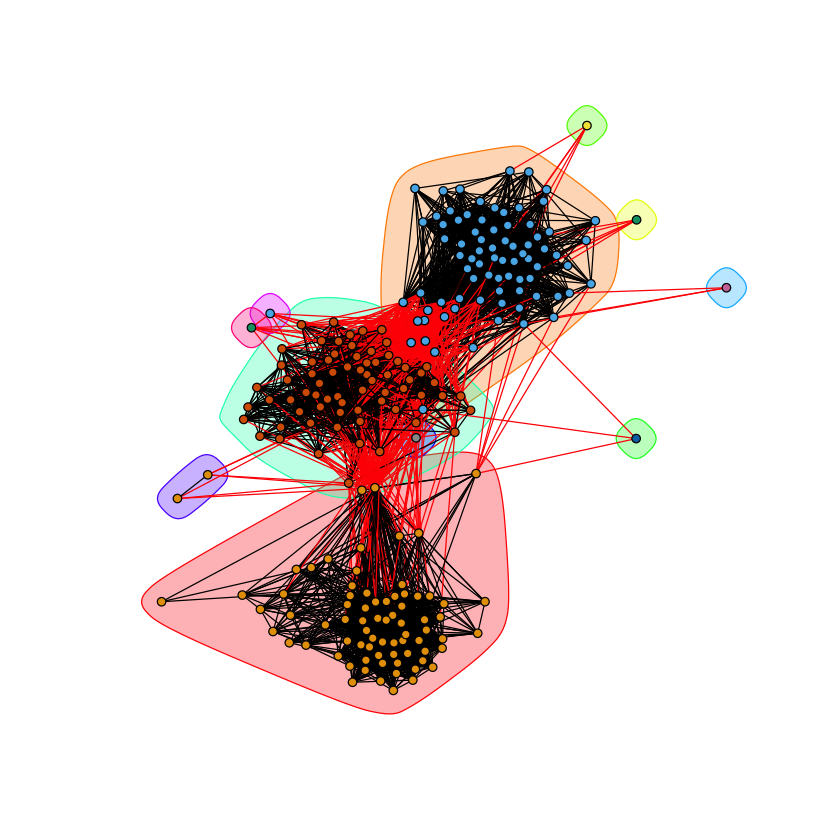
\includegraphics{Figures/1_3_2_11.png}}
\caption{community structure using Edge-Betweenness algorithms}
\label{1_3_2_11}
\end{minipage}
\end{figure}
\begin{figure}
\centering
\scalebox{0.5}{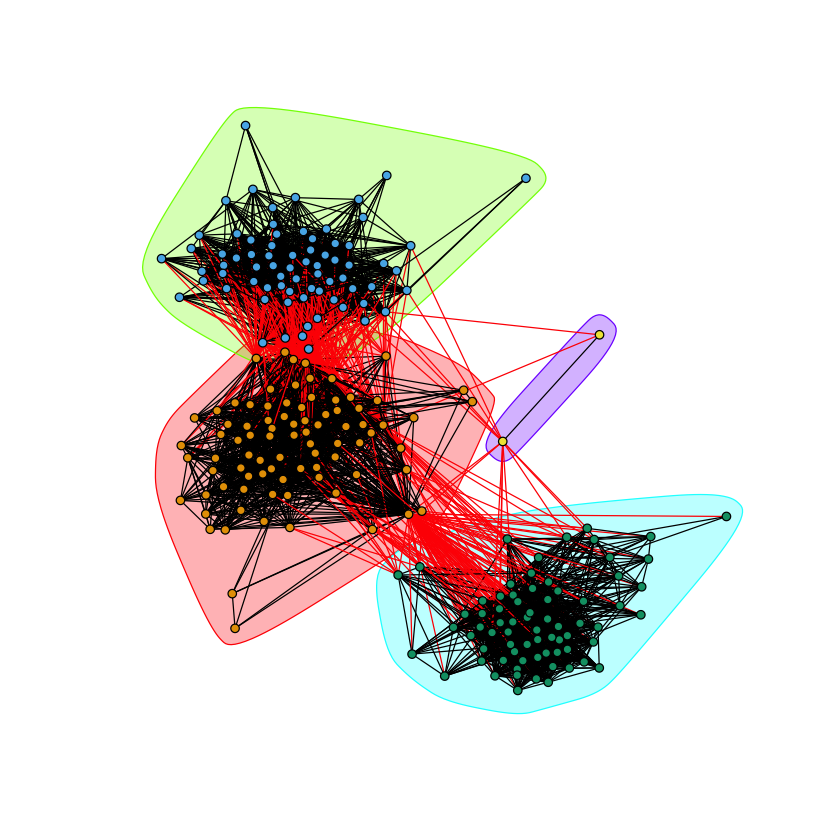
\includegraphics{Figures/1_3_2_12.png}}
\caption{community structure using Infomap algorithms}
\label{1_3_2_12}
\end{figure}

For Node ID $1087$, the community figures based on different algorithms are shown in Fig \ref{1_3_2_13}, Fig \ref{1_3_2_14} and Fig \ref{1_3_2_15}.

\begin{figure}
\centering
\begin{minipage}[t]{0.48\textwidth}
\centering
\scalebox{1}{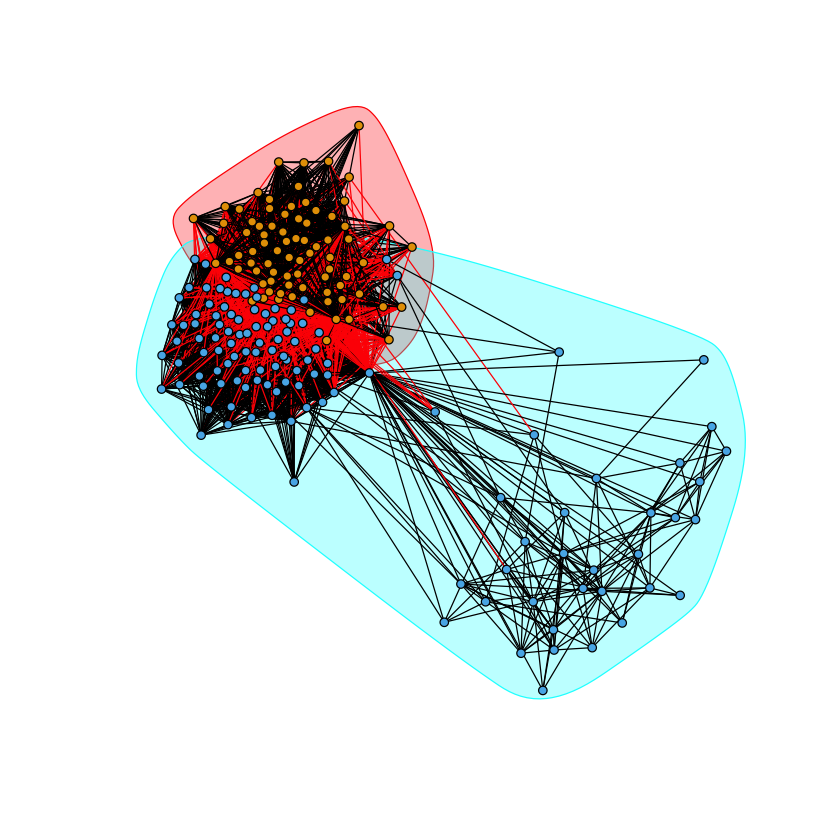
\includegraphics{Figures/1_3_2_13.png}}
\caption{community structure using Fast-Greedy algorithms}
\label{1_3_2_13}
\end{minipage}
\begin{minipage}[t]{0.48\textwidth}
\centering
\scalebox{1}{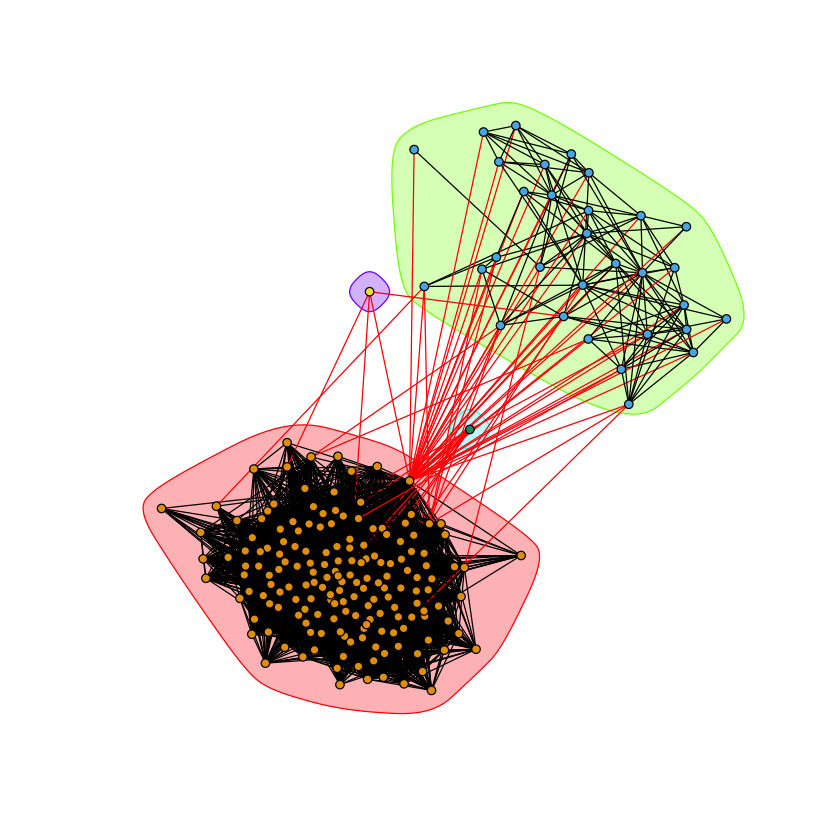
\includegraphics{Figures/1_3_2_14.png}}
\caption{community structure using Edge-Betweenness algorithms}
\label{1_3_2_14}
\end{minipage}
\end{figure}
\begin{figure}
\centering
\scalebox{0.5}{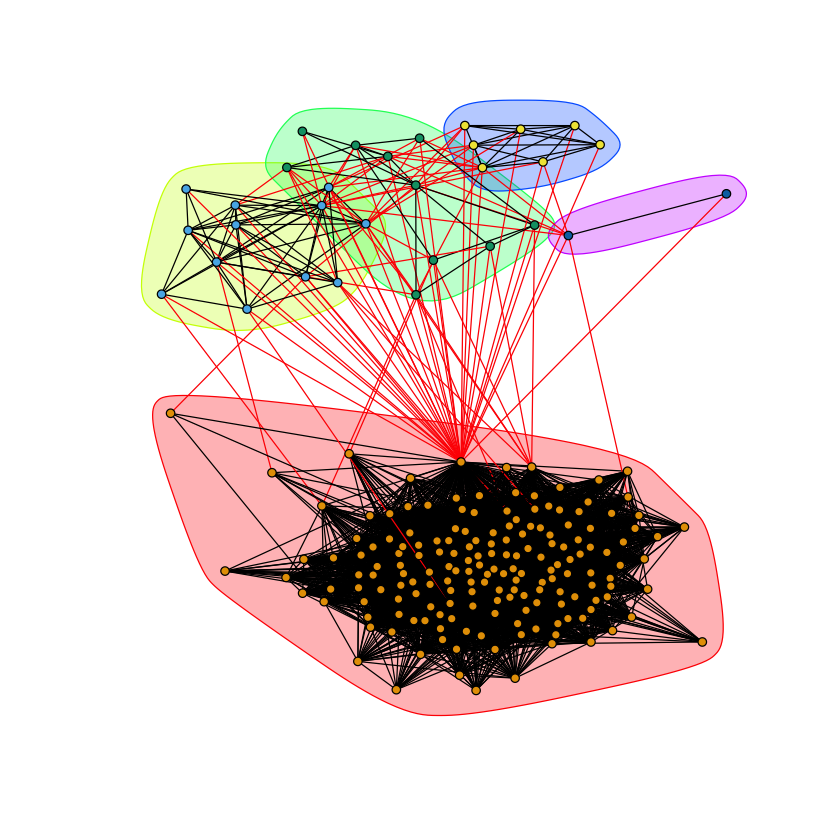
\includegraphics{Figures/1_3_2_15.png}}
\caption{community structure using Infomap algorithms}
\label{1_3_2_15}
\end{figure}

What's more, all the modularity scores from above core nodes' personalized network computed by different algorithms is shown in Table \ref{modtable2}.

\begin{table}[h]
\center
\caption{The modularity scores for core nodes' personalized network}
\begin{tabular}{c|l|l|l} 
\textbf{Node ID} & \textbf{Fast-Greedy} & \textbf{Edge-Betweenness} & \textbf{Infomap}\\\hline
$1$ & $0.44185$ & $0.41614$ & $0.41800$\\
$108$ & $0.45812$ & $0.52132$ & $0.52068$\\
$349$ & $0.24569$ & $0.15056$ & $0.24657$\\
$484$ & $0.53421$ & $0.51544$ & $0.54344$\\
$1087$ & $0.14819$ & $0.03249$ & $0.02737$\\
\end{tabular}
\label{modtable2}
\end{table}


In comparison to the results with personalized networks with the core node, almost all the networks without the core node have a little bit larger modularity scores regardless of different algorithm we used. That shows that the networks without core node have dense connections between the nodes within communities but sparse connections between nodes in different communities. Specifically, removing core node would reduce the edges between different communities, which is why they have a higher modularity scores.

\subsubsection{Characteristic of nodes in the personalized network}

We aim to explore characteristics of nodes in the personalized network using two measures. These are two measures. One is embeddedness of a node that is defined as the number of mutual friends a node shares with the core node. Another is dispersion of a node that is defined as the sum of distances between every pair of the mutual friends the node shares with the core node. The distances should be calculated in a modified graph where the node (whose dispersion is being computed) and the core node are removed.

The expression relating the Embeddedness of a node to it’s degree is given as follows.
\begin{align}
Embedd(i) = Degree (i) - 1
\end{align}

That's because, in a core node’s network, the core node connect to all nodes in the network, which means every friends a node has is a mutual friend with the core node. The embeddedness gives us a brief explanation of the connection degree between the core node and the selected node. 

For code code $1$’s personalized network, the distribution of embeddedness and dispersion is shown in Fig \ref{1_3_3_1} and Fig \ref{1_3_3_2}.

\begin{figure}
\centering
\begin{minipage}[t]{0.48\textwidth}
\centering
\scalebox{1}{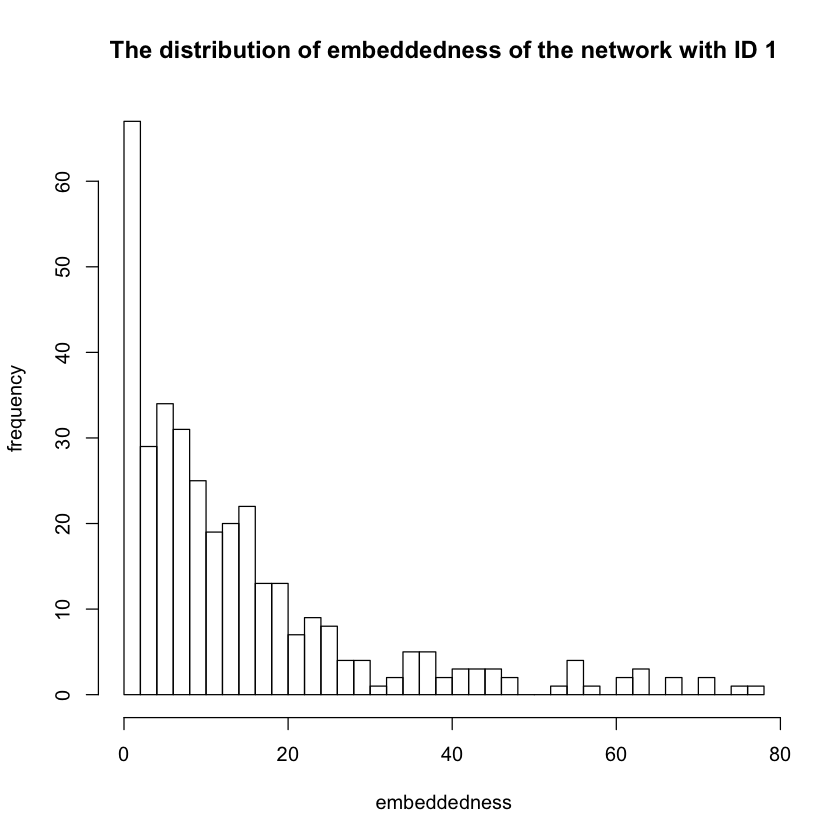
\includegraphics{Figures/1_3_3_1.png}}
\caption{The distribution of embeddedness}
\label{1_3_3_1}
\end{minipage}
\begin{minipage}[t]{0.48\textwidth}
\centering
\scalebox{1}{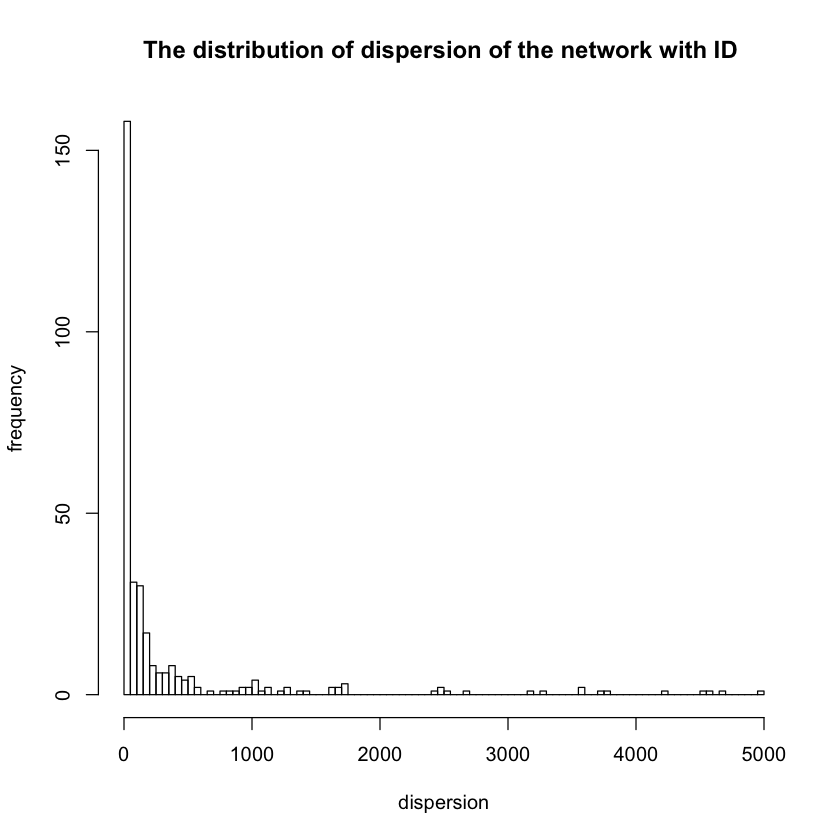
\includegraphics{Figures/1_3_3_2.png}}
\caption{The distribution of dispersion}
\label{1_3_3_2}
\end{minipage}
\end{figure}

For code code $108$’s personalized network, the distribution of embeddedness and dispersion is shown in Fig \ref{1_3_3_3} and Fig \ref{1_3_3_4}.

\begin{figure}
\centering
\begin{minipage}[t]{0.48\textwidth}
\centering
\scalebox{1}{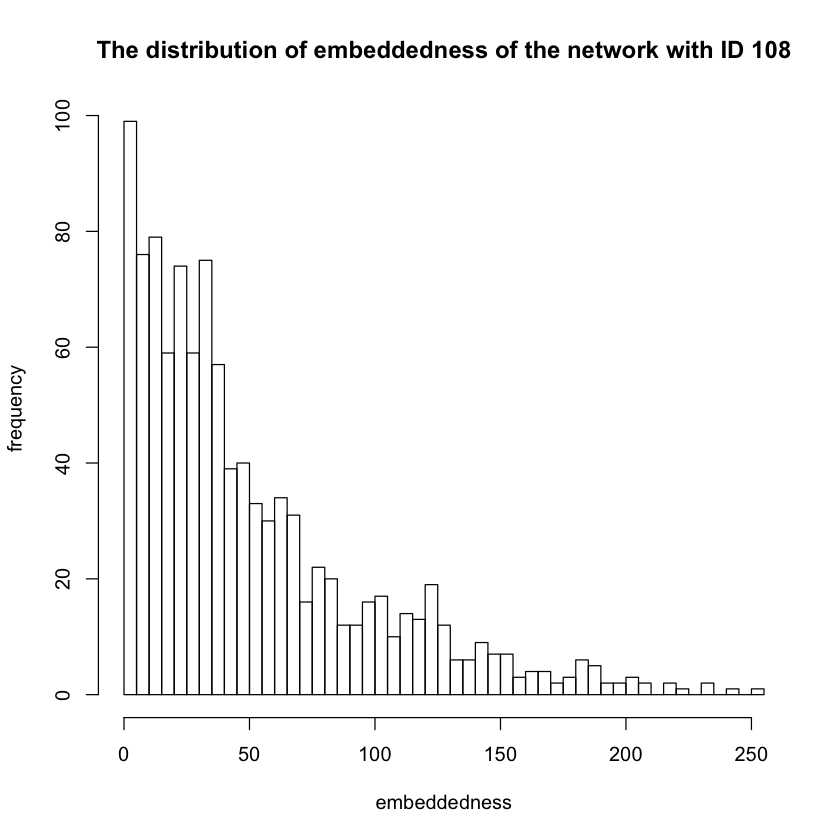
\includegraphics{Figures/1_3_3_3.png}}
\caption{The distribution of embeddedness}
\label{1_3_3_3}
\end{minipage}
\begin{minipage}[t]{0.48\textwidth}
\centering
\scalebox{1}{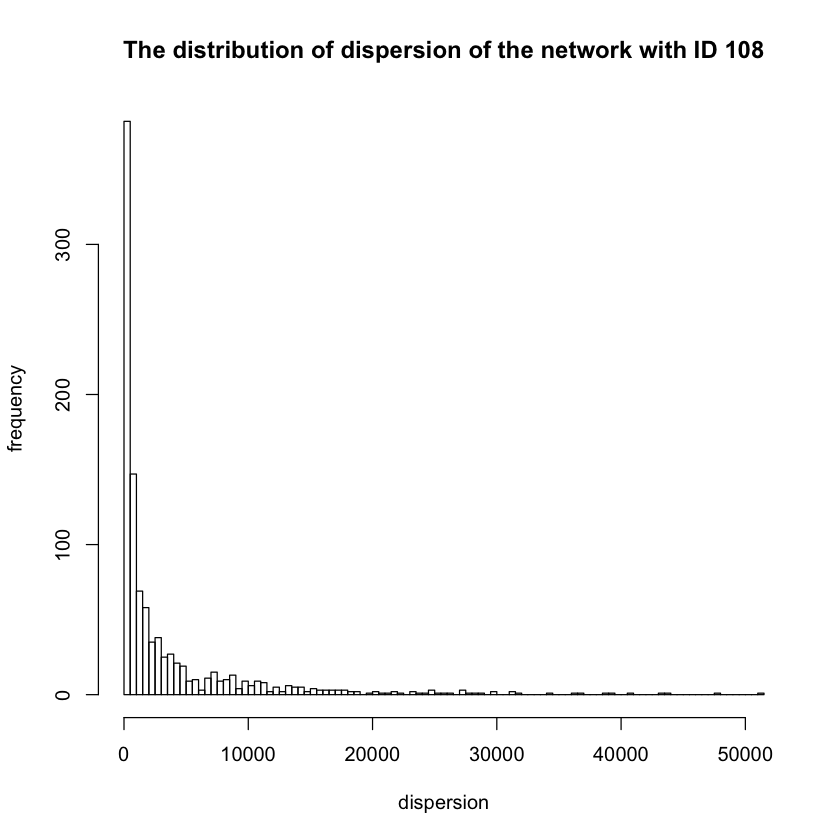
\includegraphics{Figures/1_3_3_4.png}}
\caption{The distribution of dispersion}
\label{1_3_3_4}
\end{minipage}
\end{figure}

For code code $349$’s personalized network, the distribution of embeddedness and dispersion is shown in Fig \ref{1_3_3_5} and Fig \ref{1_3_3_6}.

\begin{figure}
\centering
\begin{minipage}[t]{0.48\textwidth}
\centering
\scalebox{1}{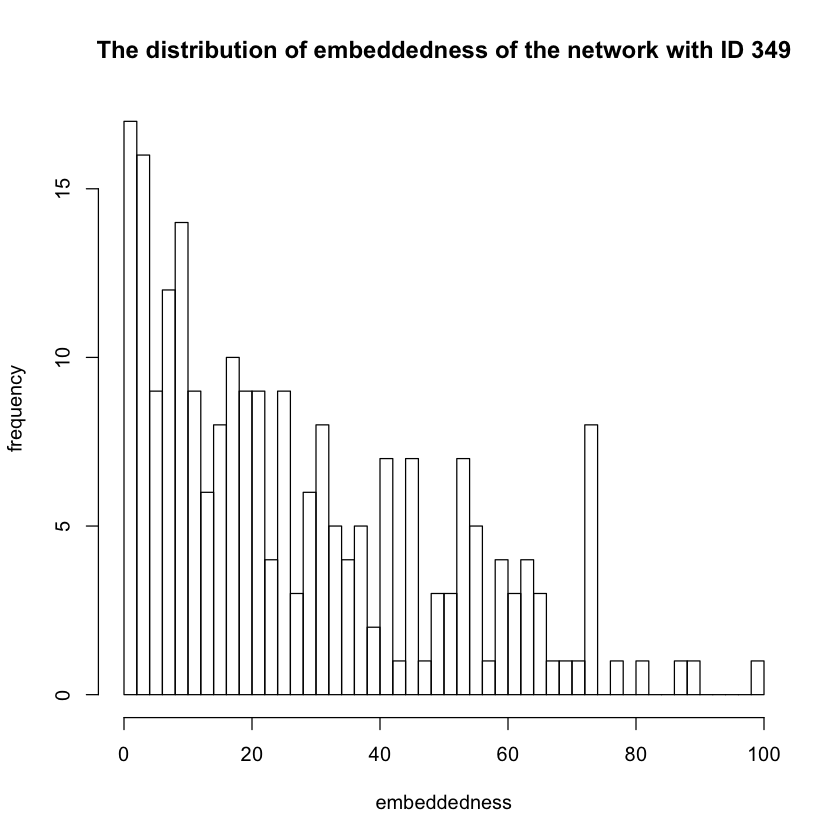
\includegraphics{Figures/1_3_3_5.png}}
\caption{The distribution of embeddedness}
\label{1_3_3_5}
\end{minipage}
\begin{minipage}[t]{0.48\textwidth}
\centering
\scalebox{1}{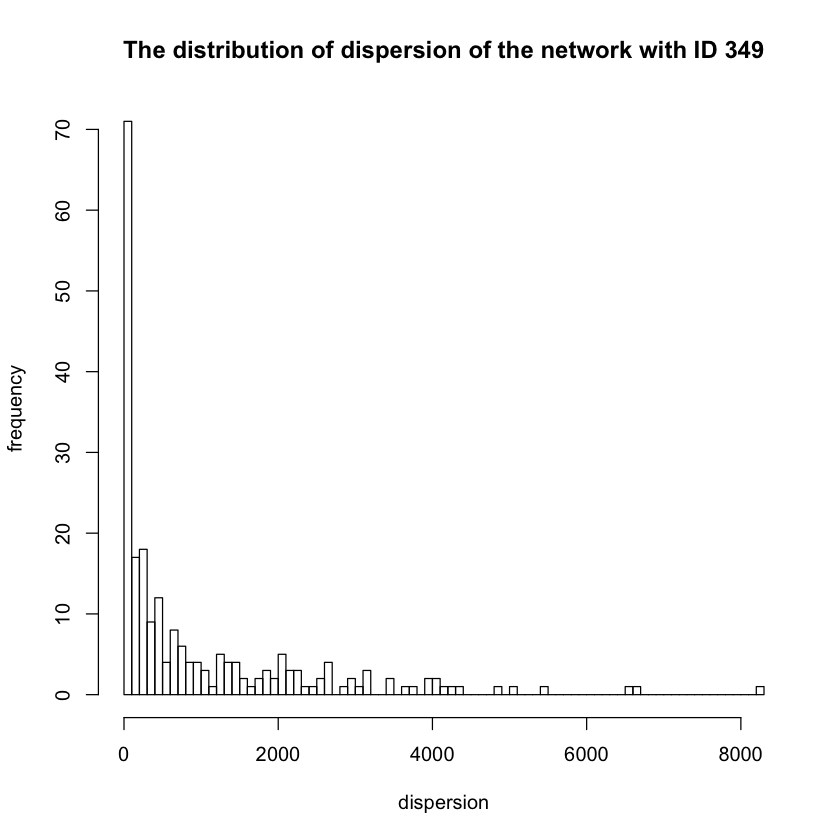
\includegraphics{Figures/1_3_3_6.png}}
\caption{The distribution of dispersion}
\label{1_3_3_6}
\end{minipage}
\end{figure}

For code code $484$’s personalized network, the distribution of embeddedness and dispersion is shown in Fig \ref{1_3_3_7} and Fig \ref{1_3_3_8}.

\begin{figure}
\centering
\begin{minipage}[t]{0.48\textwidth}
\centering
\scalebox{1}{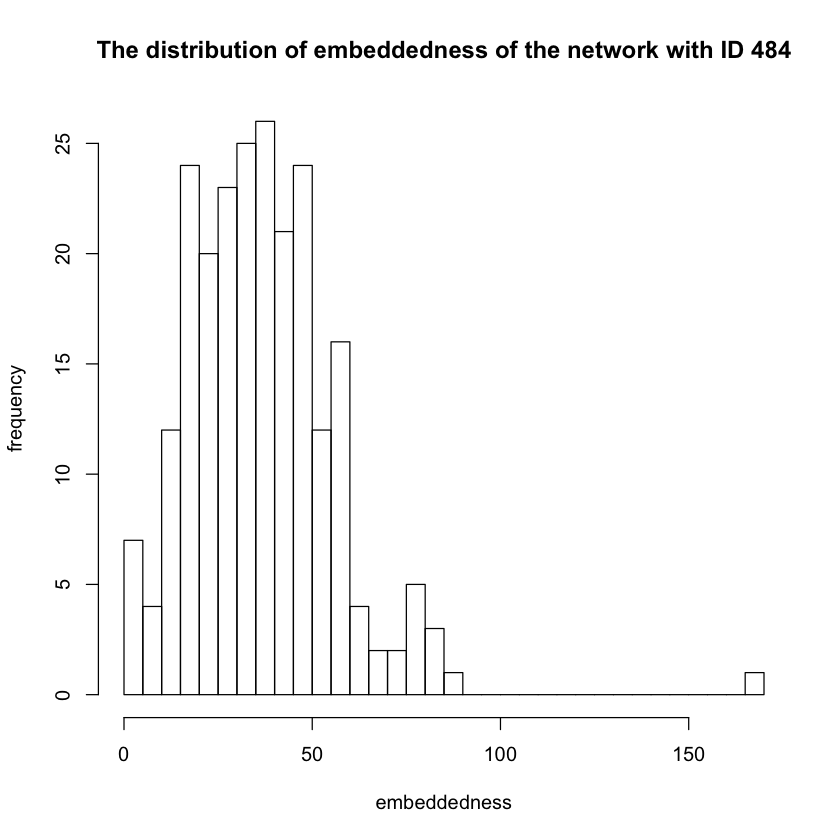
\includegraphics{Figures/1_3_3_7.png}}
\caption{The distribution of embeddedness}
\label{1_3_3_7}
\end{minipage}
\begin{minipage}[t]{0.48\textwidth}
\centering
\scalebox{1}{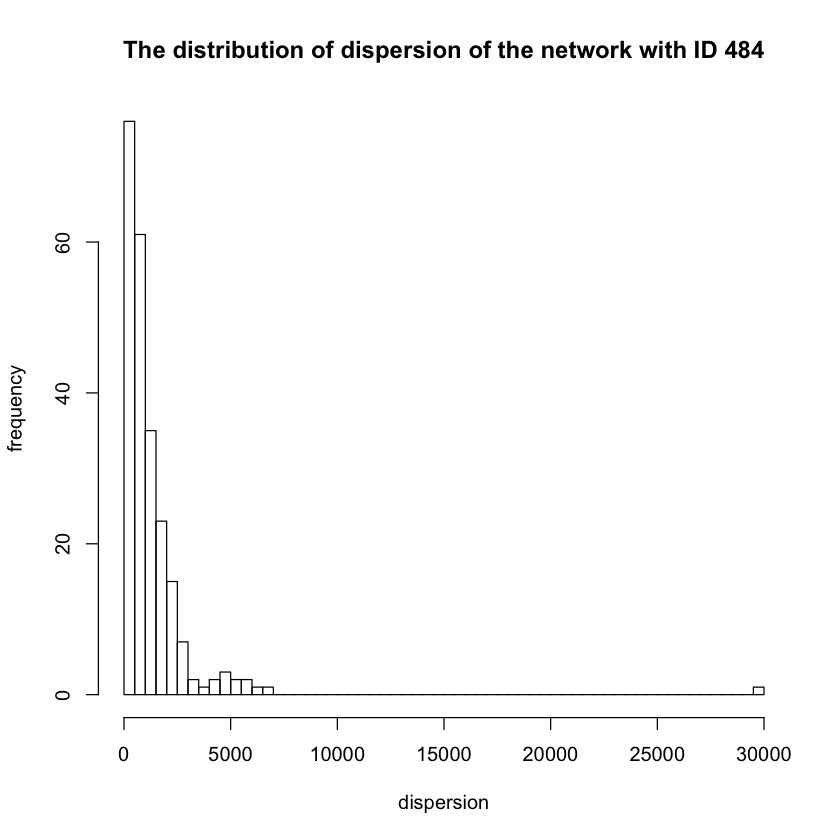
\includegraphics{Figures/1_3_3_8.png}}
\caption{The distribution of dispersion}
\label{1_3_3_8}
\end{minipage}
\end{figure}

For code code $1087$’s personalized network, the distribution of embeddedness and dispersion is shown in Fig \ref{1_3_3_9} and Fig \ref{1_3_3_10}.

\begin{figure}
\centering
\begin{minipage}[t]{0.48\textwidth}
\centering
\scalebox{1}{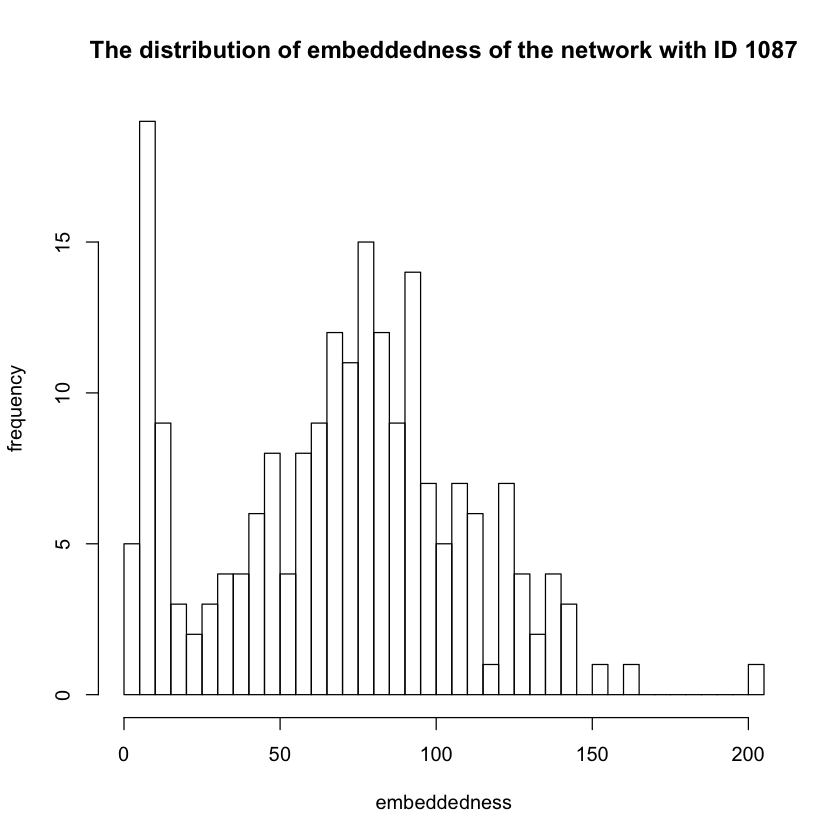
\includegraphics{Figures/1_3_3_9.png}}
\caption{The distribution of embeddedness}
\label{1_3_3_9}
\end{minipage}
\begin{minipage}[t]{0.48\textwidth}
\centering
\scalebox{1}{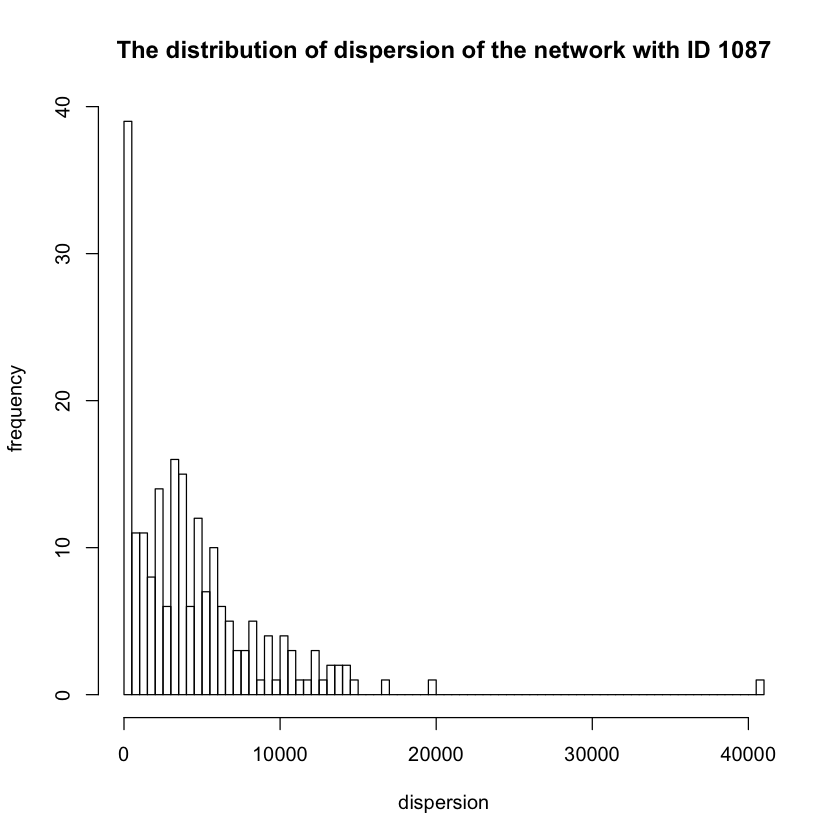
\includegraphics{Figures/1_3_3_10.png}}
\caption{The distribution of dispersion}
\label{1_3_3_10}
\end{minipage}
\end{figure}


For each of the core node’s personalized network, apply Fast-Greedy algorithm to detect the community structure of the personalized network and use colors and highlight the node with maximum dispersion and the edges incident to this node to plot this community.

For code code $1$’s personalized network, the community structure is shown in Fig \ref{1_3_4_1}.

For code code $108$’s personalized network, the community structure is shown in Fig \ref{1_3_4_2}.

For code code $349$’s personalized network, the community structure is shown in Fig \ref{1_3_4_3}.

For code code $484$’s personalized network, the community structure is shown in Fig \ref{1_3_4_4}.

For code code $1087$’s personalized network, the community structure is shown in Fig \ref{1_3_4_5}.

\begin{figure}
\centering
\begin{minipage}[t]{0.48\textwidth}
\centering
\scalebox{1}{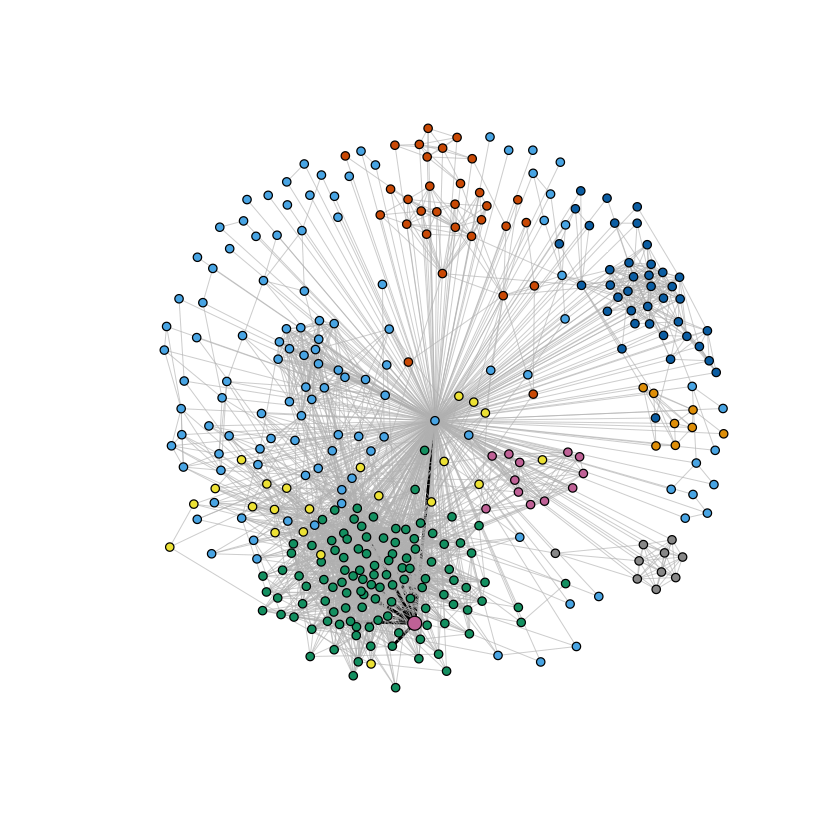
\includegraphics{Figures/1_3_4_1.png}}
\caption{The community structure of No. $1$}
\label{1_3_4_1}
\end{minipage}
\begin{minipage}[t]{0.48\textwidth}
\centering
\scalebox{1}{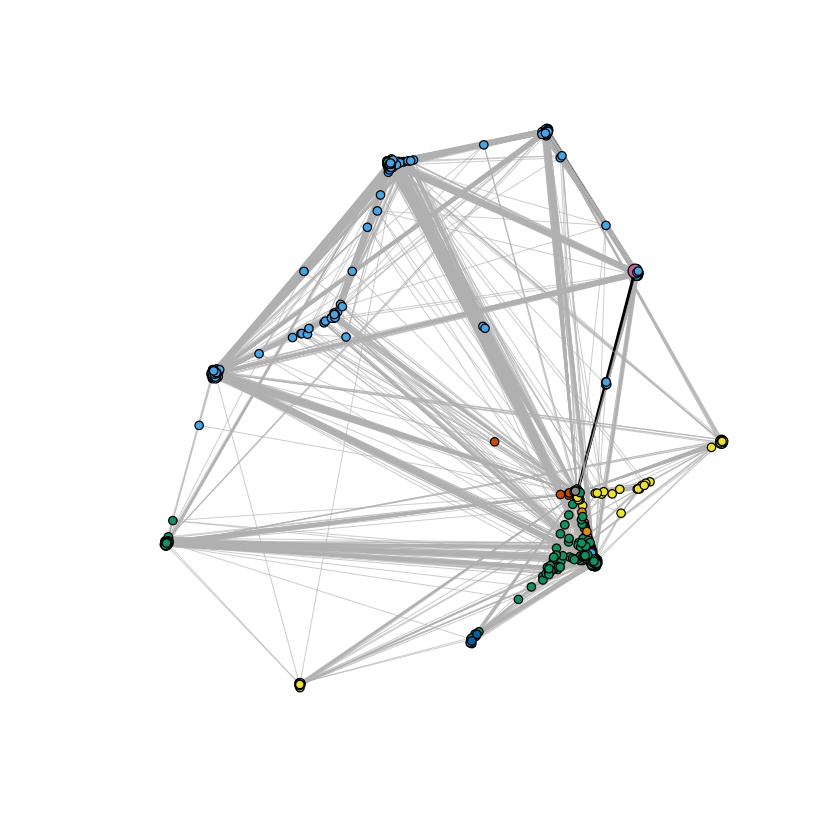
\includegraphics{Figures/1_3_4_2.png}}
\caption{TThe community structure of No. $108$}
\label{1_3_4_2}
\end{minipage}
\end{figure}

\begin{figure}
\centering
\begin{minipage}[t]{0.48\textwidth}
\centering
\scalebox{1}{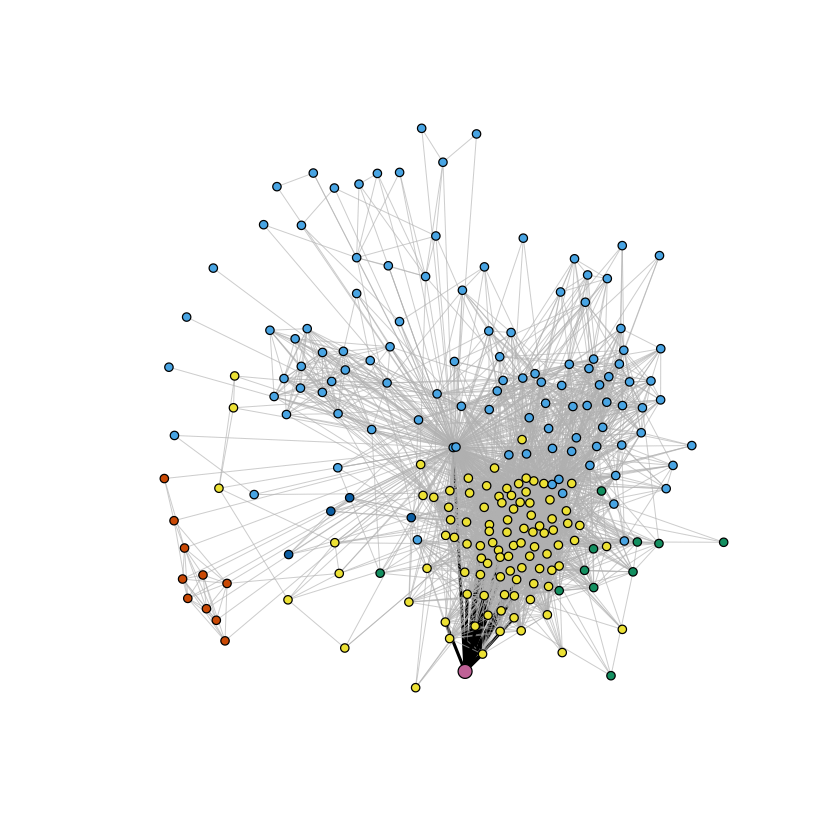
\includegraphics{Figures/1_3_4_3.png}}
\caption{The community structure of No. $349$}
\label{1_3_4_3}
\end{minipage}
\begin{minipage}[t]{0.48\textwidth}
\centering
\scalebox{1}{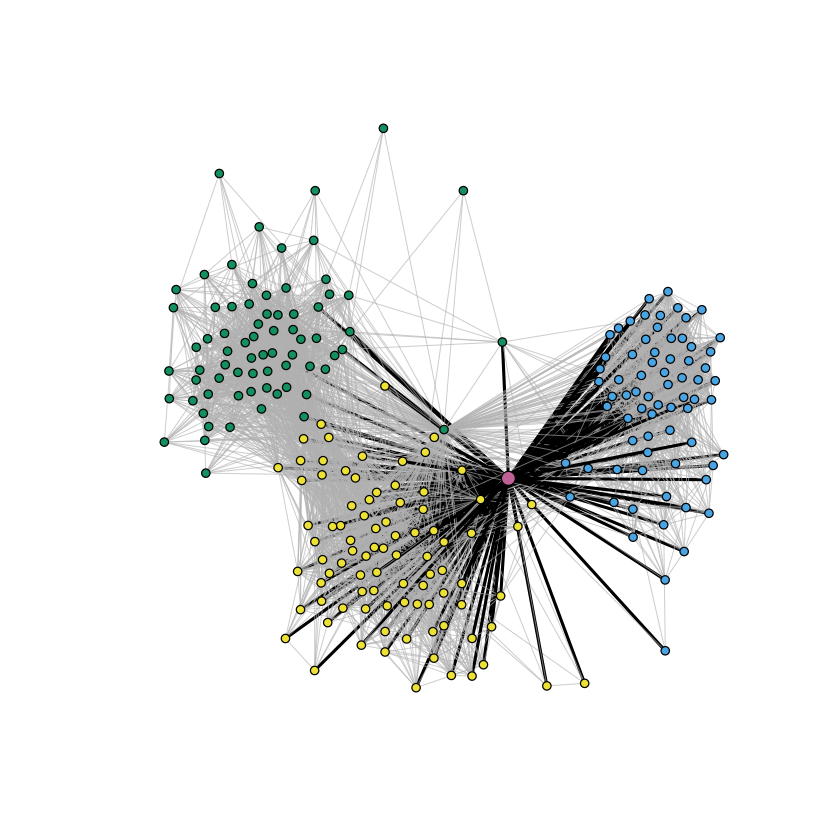
\includegraphics{Figures/1_3_4_4.png}}
\caption{The community structure of No. $484$}
\label{1_3_4_4}
\end{minipage}
\end{figure}
\begin{figure}
\centering
\scalebox{0.5}{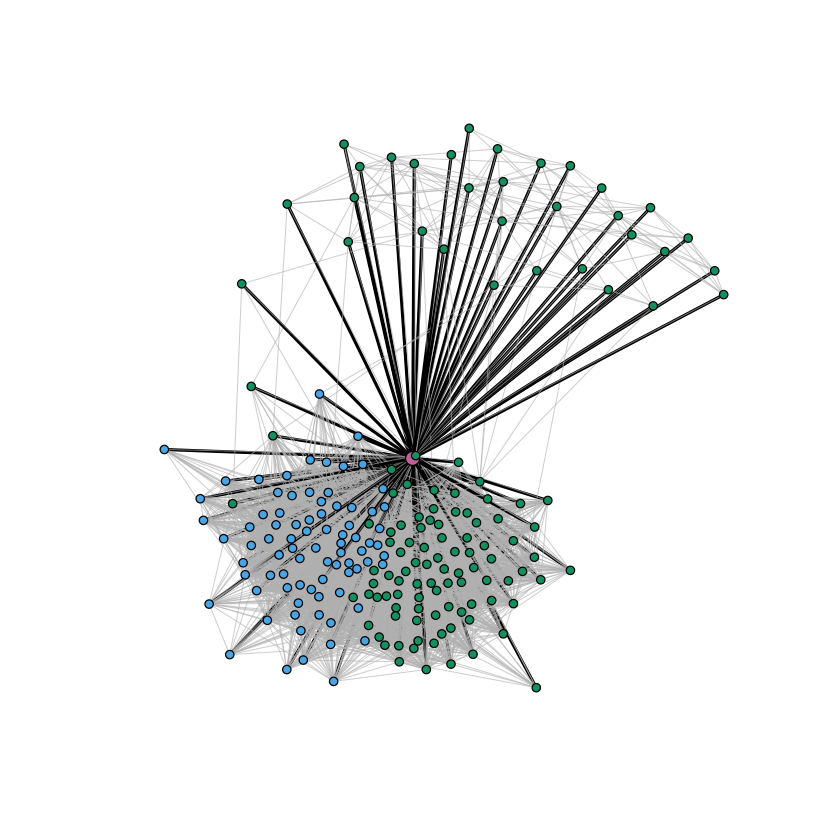
\includegraphics{Figures/1_3_4_5.png}}
\caption{The community structure of No. $1087$}
\label{1_3_4_5}
\end{figure}

Similarly, this time we highlight the node with maximum embeddedness. 

For code code $1$’s personalized network, the community structure is shown in Fig \ref{1_3_4_11}.

For code code $108$’s personalized network, the community structure is shown in Fig \ref{1_3_4_12}.

For code code $349$’s personalized network, the community structure is shown in Fig \ref{1_3_4_13}.

For code code $484$’s personalized network, the community structure is shown in Fig \ref{1_3_4_14}.

For code code $1087$’s personalized network, the community structure is shown in Fig \ref{1_3_4_15}.

\begin{figure}
\centering
\begin{minipage}[t]{0.48\textwidth}
\centering
\scalebox{1}{\includegraphics{Figures/1_3_4_11.png}}
\caption{The community structure of No. 1}
\label{1_3_4_11}
\end{minipage}
\begin{minipage}[t]{0.48\textwidth}
\centering
\scalebox{1}{\includegraphics{Figures/1_3_4_12.png}}
\caption{The community structure of No. 108}
\label{1_3_4_12}
\end{minipage}
\end{figure}

\begin{figure}
\centering
\begin{minipage}[t]{0.48\textwidth}
\centering
\scalebox{1}{\includegraphics{Figures/1_3_4_13.png}}
\caption{The community structure of No. 349}
\label{1_3_4_13}
\end{minipage}
\begin{minipage}[t]{0.48\textwidth}
\centering
\scalebox{1}{\includegraphics{Figures/1_3_4_14.png}}
\caption{The community structure of No. 484}
\label{1_3_4_14}
\end{minipage}
\end{figure}
\begin{figure}
\centering
\scalebox{0.5}{\includegraphics{Figures/1_3_4_15.png}}
\caption{The community structure of No. 1087}
\label{1_3_4_15}
\end{figure}

Still, this time we highlight the node with maximum ratio of dispersion to embeddedness. 

For code code $1$’s personalized network, the community structure is shown in Fig \ref{1_3_4_6}.

For code code $108$’s personalized network, the community structure is shown in Fig \ref{1_3_4_7}.

For code code $349$’s personalized network, the community structure is shown in Fig \ref{1_3_4_8}.

For code code $484$’s personalized network, the community structure is shown in Fig \ref{1_3_4_9}.

For code code $1087$’s personalized network, the community structure is shown in Fig \ref{1_3_4_10}.

\begin{figure}
\centering
\begin{minipage}[t]{0.48\textwidth}
\centering
\scalebox{1}{\includegraphics{Figures/1_3_4_6.png}}
\caption{The community structure of No. 1}
\label{1_3_4_6}
\end{minipage}
\begin{minipage}[t]{0.48\textwidth}
\centering
\scalebox{1}{\includegraphics{Figures/1_3_4_7.png}}
\caption{The community structure of No. 108}
\label{1_3_4_7}
\end{minipage}
\end{figure}

\begin{figure}
\centering
\begin{minipage}[t]{0.48\textwidth}
\centering
\scalebox{1}{\includegraphics{Figures/1_3_4_8.png}}
\caption{The community structure of No. 349}
\label{1_3_4_8}
\end{minipage}
\begin{minipage}[t]{0.48\textwidth}
\centering
\scalebox{1}{\includegraphics{Figures/1_3_4_9.png}}
\caption{The community structure of No. 484}
\label{1_3_4_9}
\end{minipage}
\end{figure}
\begin{figure}
\centering
\scalebox{0.5}{\includegraphics{Figures/1_3_4_10.png}}
\caption{The community structure of No. 1087}
\label{1_3_4_10}
\end{figure}

From the figure, we could find that the maximum dispersion node's neighbors are very likely not connected to each other. In other words, they are very less acquainted with each other, in term of community, which means that they supposed not to belong to same communities. But this measurement also call into question that when the pair of nodes is unconnected the shortest path would be infinity. For a real world example, a node with high dispersion is like a traveller whose friends are from all over the world.

And for the node which has the maximum embeddedness value with its core node, this node shares the most mutual friends with its core node. In other words, the node with the core node are very acquainted with each other and they share the same friends. For a real world example, a node with high embeddedness is like a roommate of core node, they go to same classes and do everything together and obviously share the same friends.

At last, when a node has the maximum ratio of dispersion to embeddedness value with its core node, this node’s dispersion is pretty large, and at the same time this node’s embeddedness is relatively small, which can be explained as that this node shares no friends with the core node but all his friends are very less acquainted with each other. For a real world example, they may be a couple and in a long distance relationship, it's obvious that they have only a few common friends with each other because they live in different place.

\subsection{Friend recommendation in personalized networks}

In this section, the network that we used is the personalized network of node with ID 415.

Question 16:

We find the list of all nodes with degree 24 within the personalized network:

Nr = [31  53  75  90  93 102 118 133 134 136 137]

The node ID is based on the personalized network. Thus, |Nr| is equal to 11.\\

Question 17:

For observing the difference of three recommendation algorithms, we ran our program many times and get an interesting result. The accuracy of these three algorithms we got are as follows: (order is: "Common Neighbors measure", "Jaccard measure", and "Adamic Adar measure")

0.8429869 0.8043000 0.8461796

0.8327922 0.7958622 0.8307468

0.8152561 0.7930083 0.8220310

0.8377378 0.8017198 0.8401728

0.8320815 0.7953243 0.8268939

0.8271593 0.8162239 0.8205897

0.8460757 0.8111159 0.8497986

As we can see, both "Common Neighbors measure" algorithm and "Adamic Adar measure" can get best results according to our experiments, but the accuracy of these two algorithm is really similar each time (sometimes "Common Neighbors measure" performs better, sometimes "Adamic Adar measure" performs better). However, "Jaccard measure" get the worst accuracy among these three algorithms. 

The reason of this might be:

(1) "Common Neighbors measure" tend to recommend high-degree nodes to objection nodes according to its definition, since high-degree nodes in network probably connect to most of other nodes within the network. This probabiliy may not seem so meaningful in real world since companies are more likely to discover potential relationships in network and make "surprising" recommendations to users. In other words, for example, if a guy is a famous people (a high-degree node in network), people probably connect with him before the recommender system recommends this famous guy to the user; so that in this way, recommend a person who is "popular" in the network may not be an impressive thing for a recommender system. So some ohter measures like "Jaccard measure" and "Adamic Adar measure" are designed to avoid this influence. However, there is no doubt that "Common Neighbors measure" will help us get good recommendations; thus it is not surprise that using "Common Neighbors measure" can get high accuracy in our problem;

(2) "Jaccard measure" is an improvement of "Common Neighbors measure", which divides the length of the union of two nodes to weaken the influence of high-degree nodes. However, during experiments I found that there are many high-degree nodes connected to our objection nodes, so this can perfectly explans why we get worse results by using "Jaccard measure", some high-degree nodes which are true neighbors before we deleted edges may have low "Jaccard measure score" because of its high-degree property.

(3) "Adamic Adar measure" is also an improment of "Common Neighbors measure", which intuitively shows that common friends who have very few friends can make more contribution to recommendation. It is easy to understand that if both people are connected to a person who may not like to connect with others, these two people must have high probability to be friends. This algorithm shows nearly equal performence with "Common Neighbors measure" in our problem. This is reasonable because when only considering the definition of the algorithm, "Adamic Adar measure score"
won't be influenced by some properties of nodes in network like "Jaccard measure".


\section{Google+ Network}

In this section, we explored a directed graph: Google+ network.

Question 18:

There are 132 personal networks in total.

There are 57 personal networks for users who have more than 2 circles.\\

Question 19:

As we can see in the following plots, the in-degree distributions of the three personal networks are different, and the out-degree distributions of the three personal networks are relatively similar (slightly different).

(1) For Nodeid: 109327480479767108490

In-degree distribution is shown in Fig \ref{2_1_1}.

Out-degree distribution is shown in Fig \ref{2_1_2}.

\begin{figure}[h]
\centering
\begin{minipage}[t]{0.48\textwidth}
\centering
\scalebox{1}{\includegraphics{Figures/2_1_1.png}}
\caption{In Degree Distribution of ID:$109327480479767108490$}
\label{2_1_1}
\end{minipage}
\begin{minipage}[t]{0.48\textwidth}
\centering
\scalebox{1}{\includegraphics{Figures/2_1_2.png}}
\caption{Out Degree Distribution of ID:$109327480479767108490$}
\label{2_1_2}
\end{minipage}
\end{figure}

(2) For Nodeid: 115625564993990145546

In-degree distribution is shown in Fig \ref{2_1_3}.

Out-degree distribution is shown in Fig \ref{2_1_4}.

\begin{figure}[h]
\centering
\begin{minipage}[t]{0.48\textwidth}
\centering
\scalebox{1}{\includegraphics{Figures/2_1_3.png}}
\caption{In Degree Distribution of ID:$115625564993990145546$}
\label{2_1_3}
\end{minipage}
\begin{minipage}[t]{0.48\textwidth}
\centering
\scalebox{1}{\includegraphics{Figures/2_1_4.png}}
\caption{Out Degree Distribution of ID:$115625564993990145546$}
\label{2_1_4}
\end{minipage}
\end{figure}

(3) For Nodeid: 101373961279443806744

In-degree distribution is shown in Fig \ref{2_1_5}.

Out-degree distribution is shown in Fig \ref{2_1_6}.

\begin{figure}[h]
\centering
\begin{minipage}[t]{0.48\textwidth}
\centering
\scalebox{1}{\includegraphics{Figures/2_1_5.png}}
\caption{In Degree Distribution of ID:$101373961279443806744$}
\label{2_1_5}
\end{minipage}
\begin{minipage}[t]{0.48\textwidth}
\centering
\scalebox{1}{\includegraphics{Figures/2_1_6.png}}
\caption{Out Degree Distribution of ID:$101373961279443806744$}
\label{2_1_6}
\end{minipage}
\end{figure}

Question 20:

1. Modularity Scores

They have different modularity scores, which means that they have different strength of division of a network into modules.

(1) for Nodeid: 109327480479767108490 Modularity Score is: 0.252765.

(2) for Nodeid: 115625564993990145546 Modularity Score is: 0.319473.

(3) for Nodeid 101373961279443806744 Modularity Score is: 0.191090.

2. The plots of the communities using colors are as below:

(1) for Nodeid: 109327480479767108490, the plot is shown in Fig \ref{2_2_1}.

(2) for Nodeid 115625564993990145546,  the plot is shown in Fig \ref{2_2_2}.

(3) for Nodeid 101373961279443806744,  the plot is shown in Fig \ref{2_2_3}. 


\begin{figure}[h]
\centering
\scalebox{0.7}{\includegraphics{Figures/2_2_1.png}}
\caption{Walktrap Community of ID $109327480479767108490$}
\label{2_2_1}
\end{figure}

\begin{figure}[h]
\centering
\scalebox{0.7}{\includegraphics{Figures/2_2_2.png}}
\caption{Walktrap Community of ID $115625564993990145546$}
\label{2_2_2}
\end{figure}

\begin{figure}[h]
\centering
\scalebox{0.7}{\includegraphics{Figures/2_2_3.png}}
\caption{Walktrap Community of ID $101373961279443806744$}
\label{2_2_3}
\end{figure}

Question 21:

Homogeneity: A community structure is of higher homogeneity if its clusters more likely contain only data points which are members of a single class. To some extent, it describes the class purity of clusters. The expression of Homogeneity is $1 - H(C|K) / H(C)$. $H(C|K)$ here describes the extent that the class distribution within each cluster belong to a single class. $H(C)$ is the maximum reduction in entropy the clustering information could provide, which is used for normalization purpose since homogeneity also depends on the size of the dataset and the distribution of class sizes. For instance, assigning each data point to a distinct cluster guarantees perfect homogeneity. In that case, each cluster trivially contains only members of a single class. In the perfectly homogeneous case (h = 0), $H(C|K)$ is zero because each cluster contains only members of a single class.

Completeness: A community structure is of higher completeness if all the data points that are members of a given class are more likely assigned to the same cluster. Completeness roughly run in the opposition to homogeneity. The expression of Completeness is $1 - H(K|C) / H(K)$. $H(K|C)$ here describes the extent that the distribution of cluster assignments within each class will be completely adjusted to just one single cluster. For instance, in the perfectly complete case (c = 0), $H(K|C)$ is zero. In this case, the class distribution within each cluster is adjusted to a single class.


Question 22:

(1) for Nodeid 109327480479767108490 

$H(C):$ 1.050779

$H(K):$ 1.005208

$H(C | K):$ 0.155636

$H(K | C):$ 0.673616 

Homogeneity: 0.851885 

Completeness: 0.329874

(2) for Nodeid 115625564993990145546 

$H(C):$ 8.465147

$H(K):$ 1.081191

$H(C | K):$ 4.639829

$H(K | C):$ 4.783148 

Homogeneity: 0.451890 

Completeness: -3.423962

(3) for Nodeid 101373961279443806744 

$H(C):$ 0.384320

$H(K):$ 0.493331

$H(C | K):$ 0.382834

$H(K | C):$ 1.235417 

Homogeneity: 0.003867 

Completeness: -1.504238

As we can see from the results above, these three personal networks’ homogeneity score is higher than completeness score.

Specifically, in the first personal network for userid=109327480479767108490, it both has highest homogeneity score and completeness score. There are three circles and their size $a[i]$ are 419, 346, 330 respectively. And there are four communities extracted by walk trap community detection algorithm, and their size $b[i]$ are 397, 288, 76, 13 respectively. The total number of unique nodes in three circles is $N = 764$ and the sum number of three circles is 1095, which means there is not much overlapping between circles. This can also be shown in the corresponding plot, the class distribution within each cluster is likely to belong to a single class, and the class distribution within each cluster is adjusted to a single class.

In the second personal network for userid = 115625564993990145546, it both has relatively low homogeneity score and completeness score compared to the first personal network. There are 31 circles and their size $a[i]$ are 489, 485, 373, 362... respectively. And there are 10 communities extracted using walk trap community detection algorithm, and their size $b[i]$ are 350, 256, 233, 40, 37, 3, 2, 1, ... respectively. The total number of unique nodes in three circles is $N = 727$ and the sum number of all circles is 6474, which means there is relatively more overlapping between circles. So the probability that a community just contains nodes belonging to a single circle is low. In terms of the completeness, the score is negative, which could be explained by considering that the size of individual communities $b[j]$ is smaller than the size of most of the circles $a[i]$, which reflects the low probability that a circle only contains nodes that belong to a single community.

In the third personal network for userid = 101373961279443806744, it also has relatively low homogeneity score and completeness score compared to the others. There are 3 circles and their size $a[i]$ are 471, 445, 430 respectively. And there are 31 communities extracted by walk trap community detection algorithm, and their size $b[i]$ are 442, 66, 13, 0, ... respectively, and 27 communities only contain one single node so most of the $C_{ji}$ which is the number of people belonging to community $j$ and circle $i$ are zero since most of the intersection of such communities and circles are empty set. As a result, there is low probability that a community just contains nodes that belongs to a single circle. In terms of the completeness, the completeness score is a negative score considering that the size of individual communities $b[j]$ is also smaller than the size of most of the circles $a[i]$, which reflects the low probability that a circle only contains nodes that belong to a single community.


\end{document}







